\chapter{Cosmic rays}
\label{ch:cosmic-rays}


\section{A brief history of cosmic-ray research}

% Observed effects of cosmic rays without special instruments, e.g. aurora.

The effects of low-energy solar cosmic rays were already seen in ancient times. This was in the form of the aurora borealis and aurora australis. Several ancient written recordings of the phenomenon \cite{stephenson2004aurora} have been found, moreover, many folk tales about this phenomenon exist. The cause of the aurorae was not known then. In 1600 Gilbert created a terrela, a sphere with a magnetic field resembling that of the Earth \cite{gilbert1893terrela}. In 1896 Birkeland \cite{lilensten2012terrella} showed that electron beams fired at a terrela were bent along the field lines to form circular regions around the magnetic poles like the aurora. The aurora appears to be caused by disturbances in the magnetosphere of the Earth. The disturbances are generally caused by solar winds. Magnetic reconnection occurs and causes charged particles to be accelerated into the atmosphere \cite{angelopoulos2008reconnection}. There the particles will excite and ionize oxygen and nitrogen atoms. When these de-excite or recombine the auroral colors are produced. An example of the aurora can be seen in \cref{fig:aurora}.

\begin{figure}
    \centering
    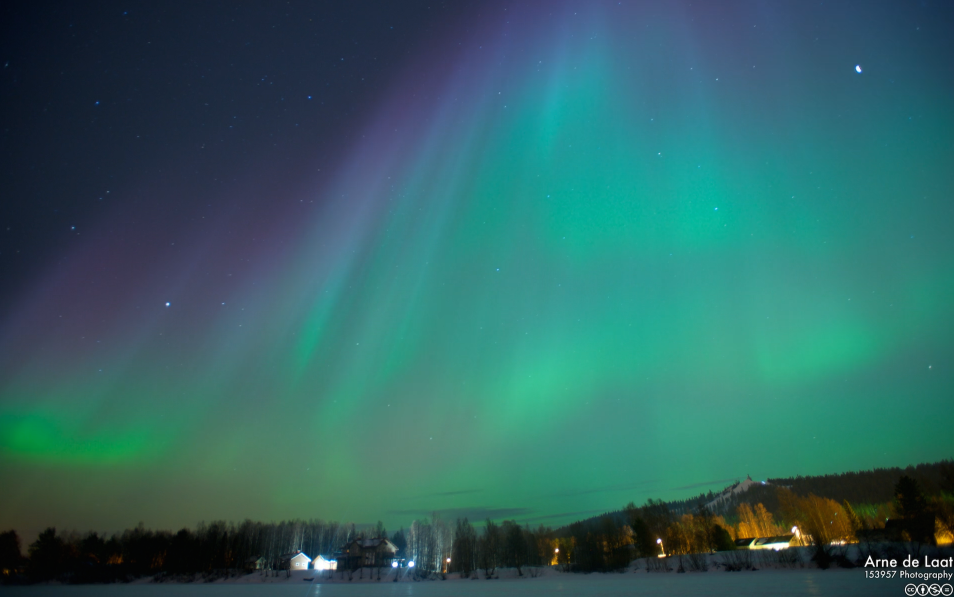
\includegraphics[width=0.6\textwidth]{plots/cosmic-rays/aurora.png}
    \caption{Aurora borealis as seen in Rovanemi, Finland on 17 March 2015, St. Patricks day. The large aurora activity on that day was due to a G4 geomagnetic storm on the sun two days earlier. The interactions between the incoming electrons and the atoms in the atmosphere creates the fluorescence. In this case the red and green colors are caused by different excitation energies in the atomic oxygen.}
    \label{fig:aurora}
\end{figure}

% Briefly talk about the discovery of the background radiation (caused by cosmic rays) and the discovery of where they come from (i.e. not radiation from Earth).
% How it was discovered that cosmic rays were charged particles.
% How this all lead to cosmic-ray research and the discovery of extensive air showers.

\subsection{Discovery of cosmic rays}

In 1785 the effects of cosmic rays were detected by de Coulomb \cite{fokkema2012} with an electroscope. An electroscope measures the amount of electrical charge in a test object. De Coulomb saw it unexpectedly discharge in the air, even though it was properly insulated. In 1895 the discovery of X-rays and their capability to ionize air \cite{flakus1981radiation} presented a good candidate for why the electroscope discharged. However, a source of the X-rays had not yet been identified. In 1896 Becquerel discovered the existence of radioactivity \cite{badash1965becquerel}. he also found that the radiation from radioactive material could cause an electroscope to discharge. Further experiments with the electroscopes were performed to assertain the source of the ionizing radiation. Experiments went over seas, underwater \cite{pacini2011sea}, underground, and far above ground \cite{angelis2013history}, but no conclusive evidence for cosmic rays was found until Hess performed balloon flights in 1911 and 1912 which accurately determined the amount of radiation at various altitudes. It showed a clear increase at very high altitudes, indicating an extra-terrestial source for the radiation. Clay \cite{clay1928latitude} found that the intensity of the ionization depended on latitude. This latitudinal dependency could be caused by the magnatic field of the Earth. Being affected by magnetic fields indicates that the particles were charged particles \cite{compton1932charged}. The indepent discovery of extensive air showers (EAS) in the atmosphere by Auger (1939) \cite{auger1939eas} and Rossi (1934) \cite{rossi1934eas} ignited the cosmic-ray research field.


\section{Cosmic ray source and their journey}

Cosmic rays are very energetic particles moving through space. Some impact Earth's atmosphere causing cascades of particles. Most commonly cosmic rays are protons, heavier atomic nuclei are the next most common component. A small fraction of the cosmic ray flux are electrons and gamma rays. Anti-particle cosmic rays have also been observed.

% What (some of) the expected origins/sources of cosmic-rays are.
The cosmic rays reaching Earth have energies anywhere from \SIrange{e9}{e21}{\eV}. Objects in space where these particles are accelerated have not yet been unequivocally identified. A strong contributing suspect are Supernova Remnants (SNR). A SNR consists of shockwaves of particles ejected by a supernova explosion. A shockwave occurs when particles are moving faster than the local speed of sound. SNRs pass through the Interstellar Medium (ISM), the region between stars in the galaxy. Here the shock picks up particles and possibly accelerates them, taking energy out of the shockwave \cite{helder2009snr}. The Fermi Large Area Telescope (LAT) discovered evidence for \Pgpz-decay in SNRs \cite{ackermann2013snr}, which is an indicator for energetic protons. Neutral pions can be created in energetic proton-proton collisions. Models predict that SNRs can contribute a significant fraction of the cosmic-ray flux up to \SI{e15}{\eV} \cite{cardillo2015snr}. Models predicting the creation of the very high energetic cosmic rays (VHECR) in Active Galactic Nuclei (AGN) and pulsars exist, but evidence for these processes has not yet been discovered.

% The acceleration mechanisms that come into play.

\subsection{Cosmic voyage}

% What the cosmic rays encounter along the way.
Cosmic rays do not travel through a perfect vacuum. The ISM is filled with particles, radiation and magnetic fields. The interstellar matter consists mainly of atomic hydrogen (\SI{70.4}{\percent} by mass), but also of helium (\SI{28.1}{\percent}), the rest (\SI{1.5}{\percent}) are heavier metals. With an average density of \SI{1}{particle\per\centi\meter\cubed} or \SI{2.7e-24}{\gram\per\centi\meter\cubed} \cite{ferriere2001ism}. Though the ISM is far from homogenous, it will be assumed for a moment. Imagine a proton travelling the diameter of the Milky Way (\SI{40}{\kilo\parsec}, or \SI{1.2e23}{\cm}) before reaching Earth. This particle will have passed through a column depth of \SI{0.324}{\gram\centi\meter\squared}. This is very small relative to the thickness of Earth's atmosphere. The thickness of the Earth's atmosphere and the mean free path of cosmic rays in it will be discussed in \cref{sec:cr:eas}.

% Explantation for the GZK cutoff/limit.
Radiation fields can in some cases affect the cosmic rays. With energies above \SI{5e19}{\eV} proton cosmic rays can interact with photons from the cosmic microwave background (CMB). In these collisions pions can be produced (via \PDelta) and the primary cosmic ray may loose up to \SI{20}{\percent} of its energy. The density of the CMB photons is \SI{550}{\per\centi\meter\cubed}. With a cross section of approximately $\sigma_{\Pproton \gamma_{CMB}} = \SI{2e-28}{\centi\meter\squared}$ at these high proton energies. This limits the possible distance from which these particles can originate and still reach Earth without undergoing this interaction. If a source of extremely energetic cosmic rays is close enough the particles may make it without undergoing these energy loss interactions. Above \SI{2e20}{\eV} the cosmic-ray flux is supressed by over a factor of 100. This upper limit of cosmic-ray energy is known as the Greisen Zatsepin Kuzmin (GZK) limit \cite{zatsepin1966gzk,greisen1966gzk}.

% How the direction of cosmic rays no longer points to their origin, gyro radius.
Cosmic rays do not simply travel in a straight line from their source to Earth. Moving charged particles are affects by magnetic fields. The Lorentz force may change the direction of the particle. The strength of this depends on the angle between the direction of motion and magnetic field lines. The deflection is strongest when the field is perpendicular to the direction of motion. The strength of all magnetic fields in the universe is not known. The overal field strength and distribution of large scale random fields for the Milky Way are being determined from experiments. The average magnetic field strength is \SI{0.6 \pm .2}{\nano\tesla} \cite{jansson2010magnetic}. The radius of curvature for relativistic particles traveling through a magnetic field is called the Larmor radius (or gyro radius). This is given by

\begin{equation}
    R = \SI{108}{\kilo\parsec}
        \frac{E_{\si{\exa\eV}}}{Z B_{\si{\nano\tesla}}}
\end{equation}

where $R$ is the radius of curvature, $Z$ the atomic number of the particle, which is equal to the charge because atomic cosmic rays are fully ionised, $B$ is the magnetic field strength, and $E$ the energy of the particle. In \cref{fig:gyroradius} the gyroradius of a proton cosmic ray is shown for various energies of the cosmic ray and various strengths of the magnetic field \cite{grigat2011anisotropy}.

\begin{figure}
    \centering
    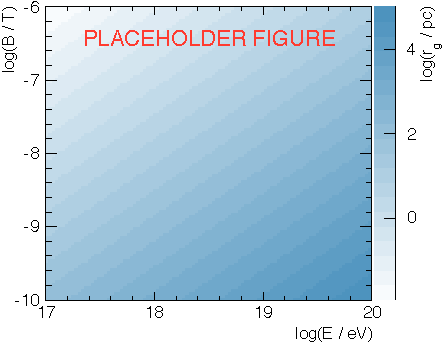
\includegraphics[width=0.6\textwidth]
                    {plots/cosmic-rays/gyroradius}
    \caption{The gyro radius of primary proton cosmic rays as a function of their energy for different magnetic field strengths. The amount of deflection greatly depends on the actual average magnetic field strength in the Milky Way, which is not precisely known. Indicated are sizes of important astronomical objects.}
    \label{fig:gyroradius}
\end{figure}

% This leads to isotropy at low energies, and possibly anisotropy at very high energies.
If the energy of a cosmic ray is low enough it may be captured by a galaxy. This can happen if the gyro radius is significantly smaller than the object. For the Milky Way this transition is around \SIrange{e16}{e18}{\eV}. For particles at and below these energies the paths though the ISM will not be straight. The deflections will cause the directions of the particles at Earth to be randomised, i.e. isotropically distributed. At low enough energies the particles are also affected by the solar wind, a cause for possible anisotropy. Above these energies, the particle paths will be straighter. Unless it encounters strong local fluctuations in the magnetic field. For cosmic rays of high enough energy anisotropy may be expected if there are clearly defined sources on the sky.

Heavy particles have smaller gyro radii and are therefore more easily contained. Consequently, heavy particles may be accelerated to higher energies at their source, being contained until accelerated to high enough energies to escape. The cosmic rays of energies above this transition can escape from the Milky Way. Similarly cosmic rays in other galaxies can escape if they have enough energy. From observations the average magnetic field strength in other visible spiral galaxies is on average \SI{.9 \pm .3}{\nano\tesla} \cite{jansson2010magnetic}. In the intergalactic medium (IGM) the particle density is approximately \SIrange{0.1}{0.25}{\per\meter\cubed} \cite{copi1995igm}. The expected average magnetic field strength in the IGM is \SI{< e-4}{\nano\tesla} \cite{kronberg1994igm}.

Knowledge about the exact distribution, strength, direction, and changes over time of the magnetic fields in the universe are not at out disposal. This makes it difficult/impossible to fully reconstruct the path of arriving cosmic rays.


\subsection{Final destination}

% Explain what cosmic rays are seen at Earth, as observed by experiments.
% How various models explain the spectrum; different compositions, galactic, extra-galactic.
At Earth cosmic rays arrive from all directions. On average the flux as a function of different energies is constant. In \cref{fig:spectrum} the measured differential flux of cosmic rays at the top of the atmosphere is shown. At low energies the flux varies over time due to solar modulation. The solar cycle of \SI{11}{\year} affects the flux in this energy region of cosmic rays. The top axis shows the equivalent center of mass collision energies. This can be used to relate the energy in the cosmic ray collision to the collision energies reported for particle colliders on Earth. At the 'end' of the spectrum, around \SI{e20}{\eV} the spectrum steepens and seems to end. No cosmic rays above $E = \SI{e21}{\eV}$ have yet been detected. The reasons for this is probably the GZK limit explained earlier. But may also be explained by the lack of sources being able to produce such highly energetic particles.

\begin{figure}
    \centering
    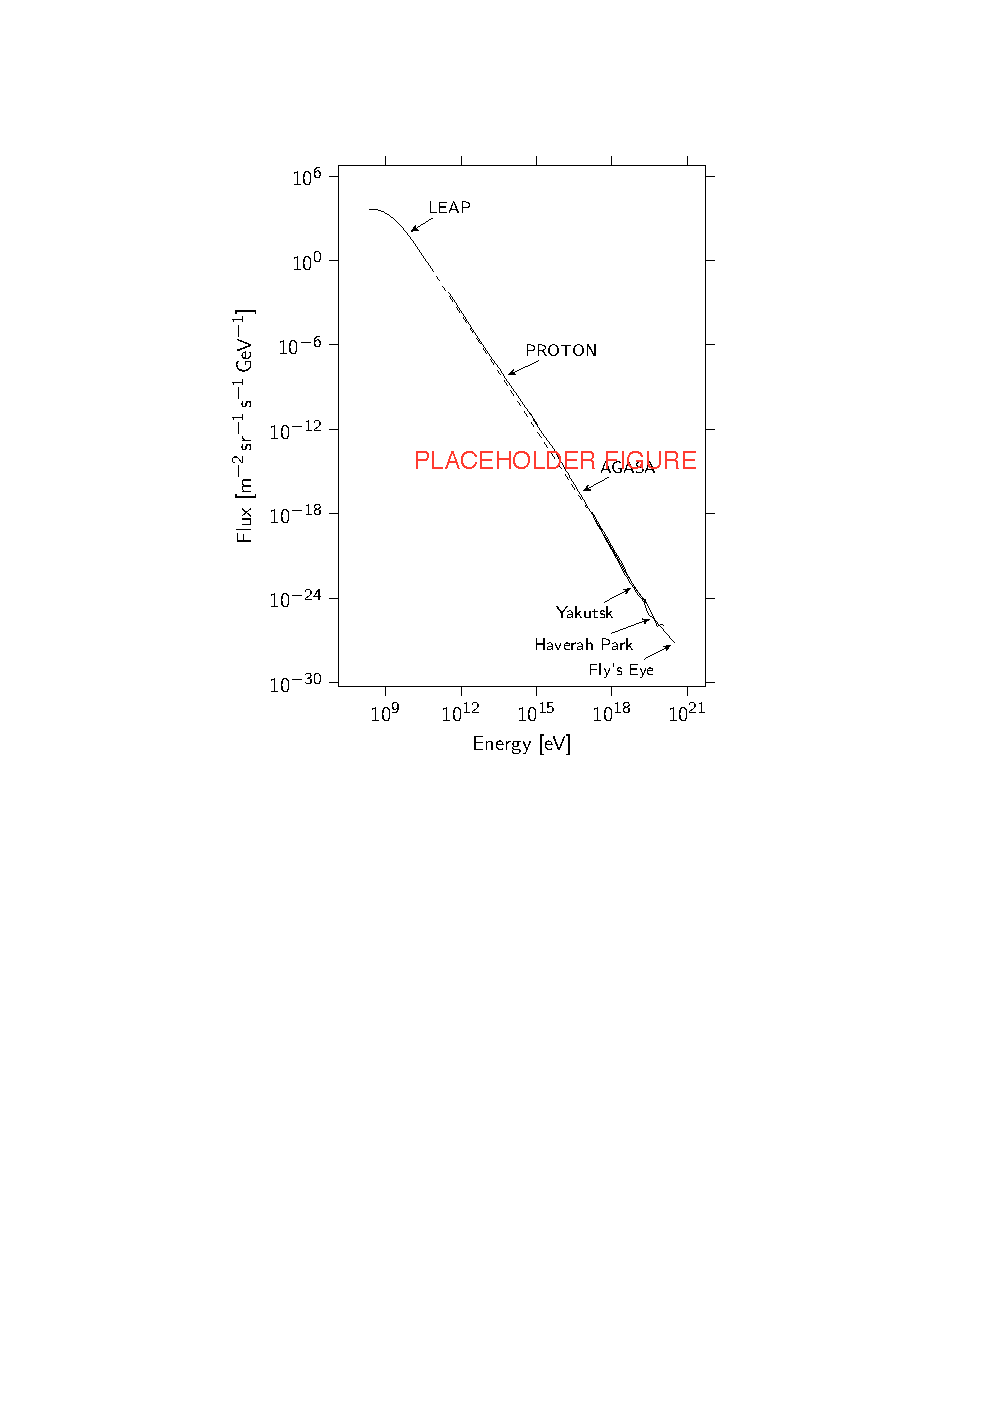
\includegraphics[width=0.6\textwidth]{plots/cosmic-rays/spectrum.pdf}
    \caption{Differential flux of primary cosmic rays versus the kinetic energy per particle. The spectral index of the spectrum is approximately $\gamma = 2.7$. Around $E = \SI{e15}{\eV}$ is the transition from directly (lower energies) to indirectly (higher energies) detected cosmic rays. At low energies the flux is indicated by a band because it changes over time due to solar modulation. Less low energy cosmic rays are observed during high solar activity. [Todo:] Equivalent center of mass collision energies as top x-axis. Marked are the achieved p-p (and p-Pb) collision energies in colliders. The transition from Galactic and extra-Galactic is determined from the expected gyro radii in the Milky Way. Also shown are likely source contributions at some energies (SNR).}
    \label{fig:spectrum}
\end{figure}


% Explain the possibilities of direct detection of cosmic rays: Low energy, balloon, space.
Cosmic rays can be detected in multiple ways. Either by detecting them directly or indirectly. In order to directly detect cosmic rays the detector needs to be above or high in the Earth's atmosphere (above \SI{25}{\kilo\meter}). This is typically done by balloon-borne experiments or space-based missions. Due to the low flux of high energy cosmic rays these methods are mainly aimed at the lower energies ($E < \SI{e15}{\eV}$). For cosmic rays of higher energies the particle cascades they create in the atmosphere are used. These cascades can be detected from the ground. The physics and characteristics of these particle showers are discussed further in \cref{sec:cr:eas}.

\subsection{Direct detection}

% What is learned from direct detection experiments: Composition, Solar modulation, van Allen belt, heliosphere, particle-antiparticle fraction, isotropy.
Being able to directly detect the particle has the advantage of easy particle identification. The main downside is the flux of cosmic-rays decreases steeply when looking at higher-energy cosmic rays. Ideally the detector has a large detection area and a very long exposure time. Unfortunately a detector that has to be flown to the top of the atmosphere or in space can only be so big before it costs too much to launch. Balloon experiments are often short runs where the balloon carrying the detector stays up for about a week. The JACEE \cite{asakimori1998jacee} and RUNJOB \cite{hareyama2011runjob} experiments flew multiple times. Each experiment reached a total fly time of \SI{60}{\day}. Notable space-based missions are PAMELA \cite{adriani2014pamela}, in orbit on the Resurs DK1 sattelite since 2006, and the AMS-02 \cite{casaus2014ams} experiment attached to the International Space Station (ISS) since 2011. These space-based experiments have been operating for many years. The measurements provide good resolution on the composition of cosmic rays at energies upto the knee \cite{amenomori2008knee}. At the knee the spectral index of the cosmic ray flux changes from $\gamma = 2.7$ to 3.1.

These experiments are able to measure the modulation of the low-energy cosmic-ray flux due to the solar activity. During high solar activity (many sunspots) the flux of galactic cosmic rays at Earth is reduced \cite{adriani2013modulation}. This is the reason for the band seen at low flux in \cref{fig:spectrum}. Also the ratio of normal and anti-particles has been determined. For electrons about \SI{15}{\percent} of the particles around \SI{e11}{\eV} are positrons \cite{aguilar2013positrons}. The \APproton/\Pproton fraction settles around \SI{2e-2}{\percent} for energies above \SI{e10}{\eV} \cite{kappl2015antiproton}. No anisotropy has been found in the arrival directions of \APelectron\Pelectron cosmic rays detected by these experiments \cite{panico2015isotropy}.

Together these direct detection experiments provide a very detailed picture of the low energy cosmic-ray spectrum. The per-nucleus spectrum of such experiments is shown in \cref{fig:PDG_28_1_fluxes_per_nucleus}.

\begin{figure}
    \centering
    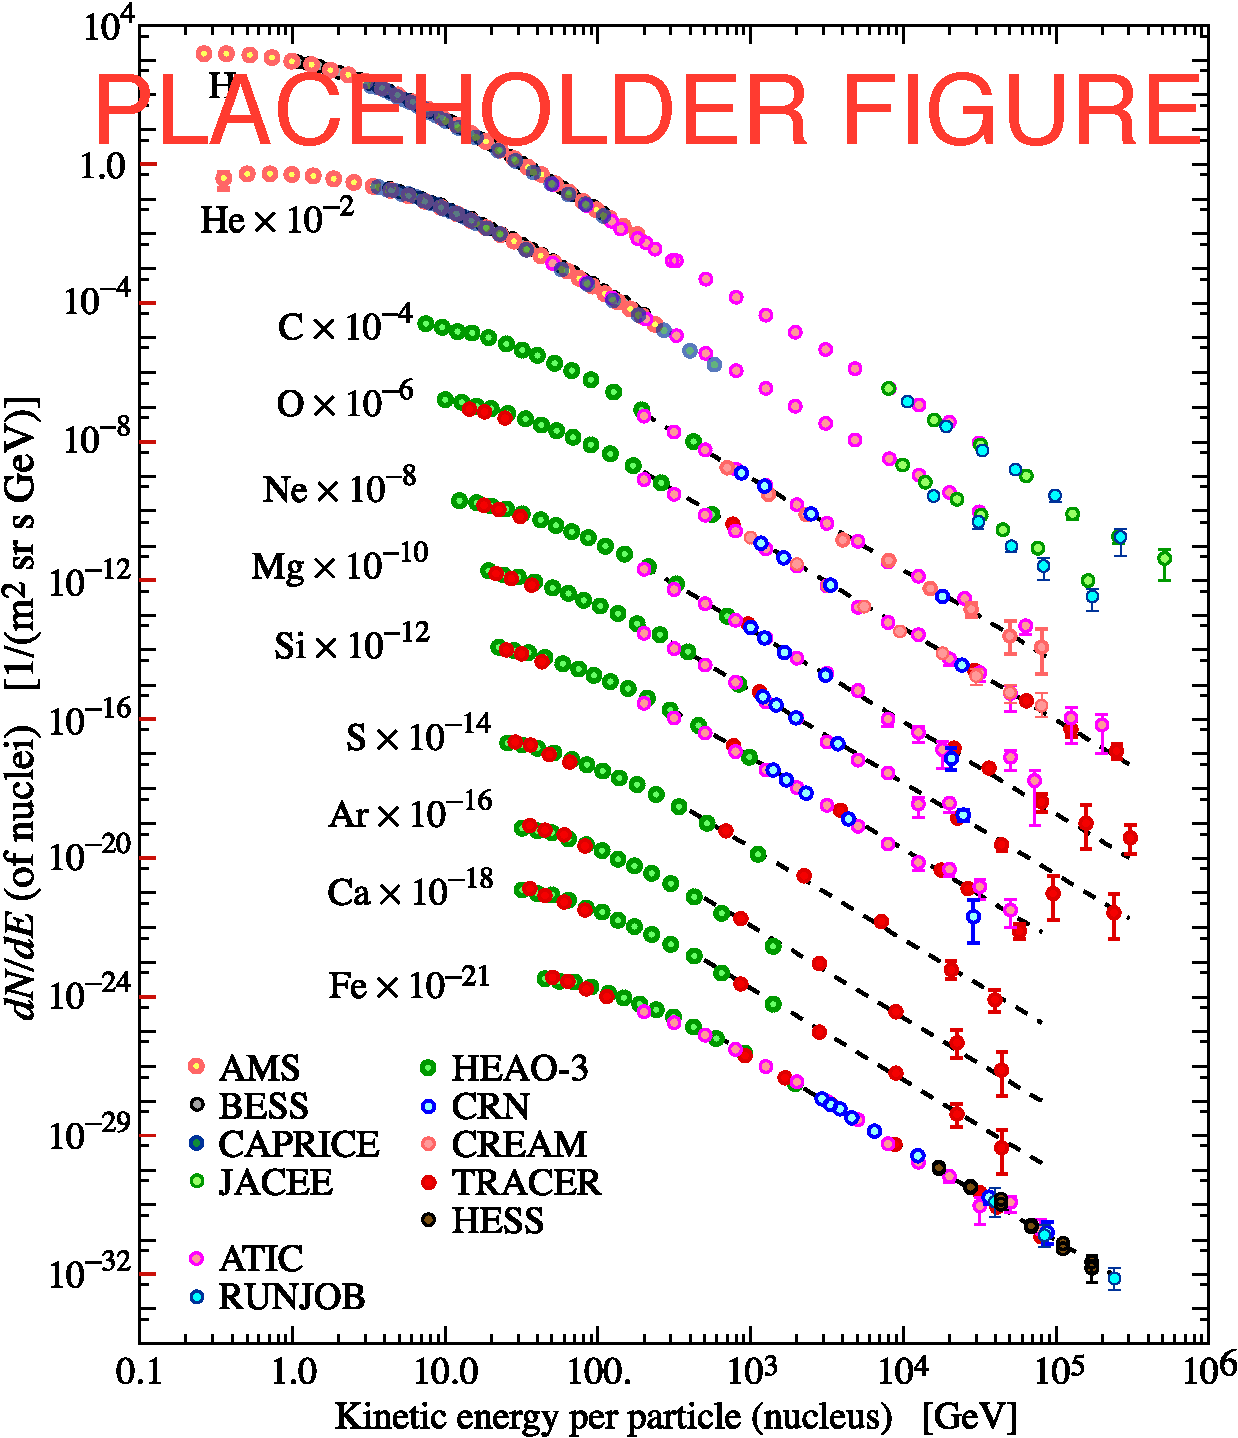
\includegraphics[width=0.6\textwidth]
                    {plots/cosmic-rays/PDG_28_1_fluxes_per_nucleus.pdf}
    \caption{Decomposed differential flux of primary cosmic rays. Balloon and space experiments directly detecting cosmic-rays provide composition data for the cosmic-rays.}
    \label{fig:PDG_28_1_fluxes_per_nucleus}
\end{figure}

The longest running space-based cosmic-ray experiments are the Voyager spacecrafts. The Pioneer probes, also carrying a cosmic-ray detector, were launched about 4 years earlier, but contact with them was lost over a decade ago. The Voyager spacecrafts were launched in 1977 to use the planetary alignment to accelerate with several gravity assists \cite{stone1977voyager}. In August 2011 Voyager I seems to have reached the heliopause of the solar system, at \SI{121}{\astronomicalunit} distance to the Sun. Here the detection rate of particles caused by the solar wind (>\SI{5e8}{\eV}) decreased steeply and the rate of cosmic-ray particles from outside the solar system (>\SI{7e10}{\eV}) increased significantly \cite{stone2013voyager}. The measurements from Voyager I are shown in \cref{fig:voyager_heliosphere}. Cosmic rays of these energies are thought to originate from supernovae in this galaxy.

\begin{figure}
    \centering
    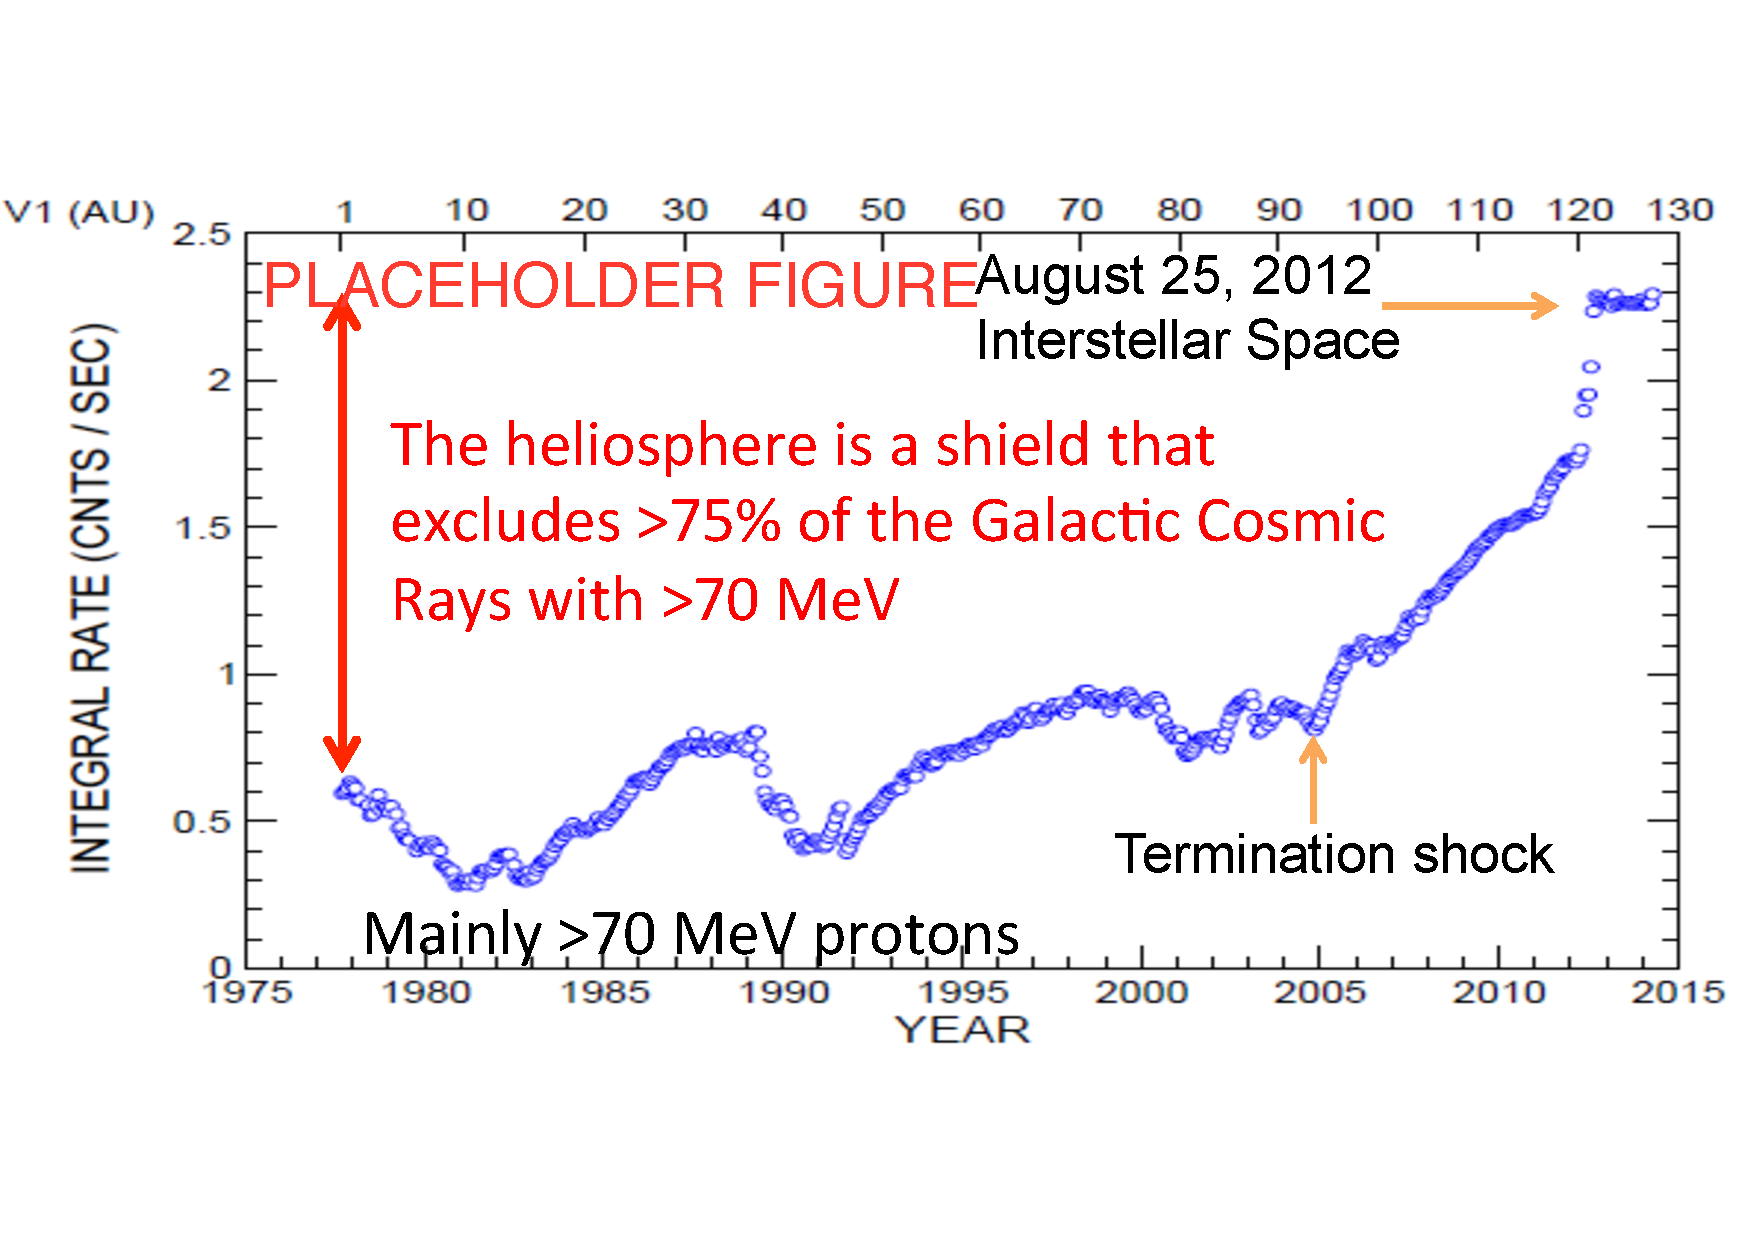
\includegraphics[width=0.6\textwidth]
                    {plots/cosmic-rays/voyager_heliosphere}
    \caption{Extrasolar cosmic ray rate by Voyager 1, stone2015]
Timeline of the cosmic ray rate measured by the Voyager 1 spaceprobe. The rate started to increase when it passed the termination shock. After passing the heliopause the rate has stabilized at 4 times the rate inside the heliosphere. This is a measure of the cosmic ray rate unaffected by solar winds.}
    \label{fig:voyager_heliosphere}
\end{figure}


\subsection{Indirect detection}

% How high-energy cosmic rays may hold information about anisotropies and possible sources (hot spot).

Currently the two biggest ground-based cosmic-ray experiments are the Pierre Auger Observatory (Auger) \cite{abraham2004auger} in Argentina and the Telescope Array (TA) \cite{abu-zayyad2012ta} in Utah. Both use particle detectors and fluorescence detectors overlooking the particle detector area. Auger has been expanded with radio detectors. Because of their size (\SI{3000}{\kilo\meter\squared} and \SI{700}{\kilo\meter\squared} respectively). and separation between the particle detectors (\SI{1.5}{\kilo\meter} and \SI{1.2}{\kilo\meter}) these experiments are looking for cosmic-rays at the highest energies. The minimum energy threshold for both experiments, ignoring the smaller low energy extensions, is above \SI{e18}{\eV}. Several cosmic-rays of $E > \SI{e20}{\eV}$ have been detected by both epxeriments, settings limits on the high-energy cosmic ray spectrum and probing the GZK limit. At these high energies possibilities for anisotropy exist. In \cref{fig:skymap_ta_auger} a combined sky map of cosmic rays detected by both experiments shows a dipole moment deviations from isotropy \cite{abbasi2015combined}. When considering only primaries with energies above $\SI{57e18}{\eV}$ the TA sees a slight preference for cosmic rays from a region on the sky, shown in \cref{fig:hotspot_ta} \cite{ta2014hotspot}. However, with a significance of $3.4 \sigma$ more data is needed to verify the excess.

\begin{figure}
    \centering
    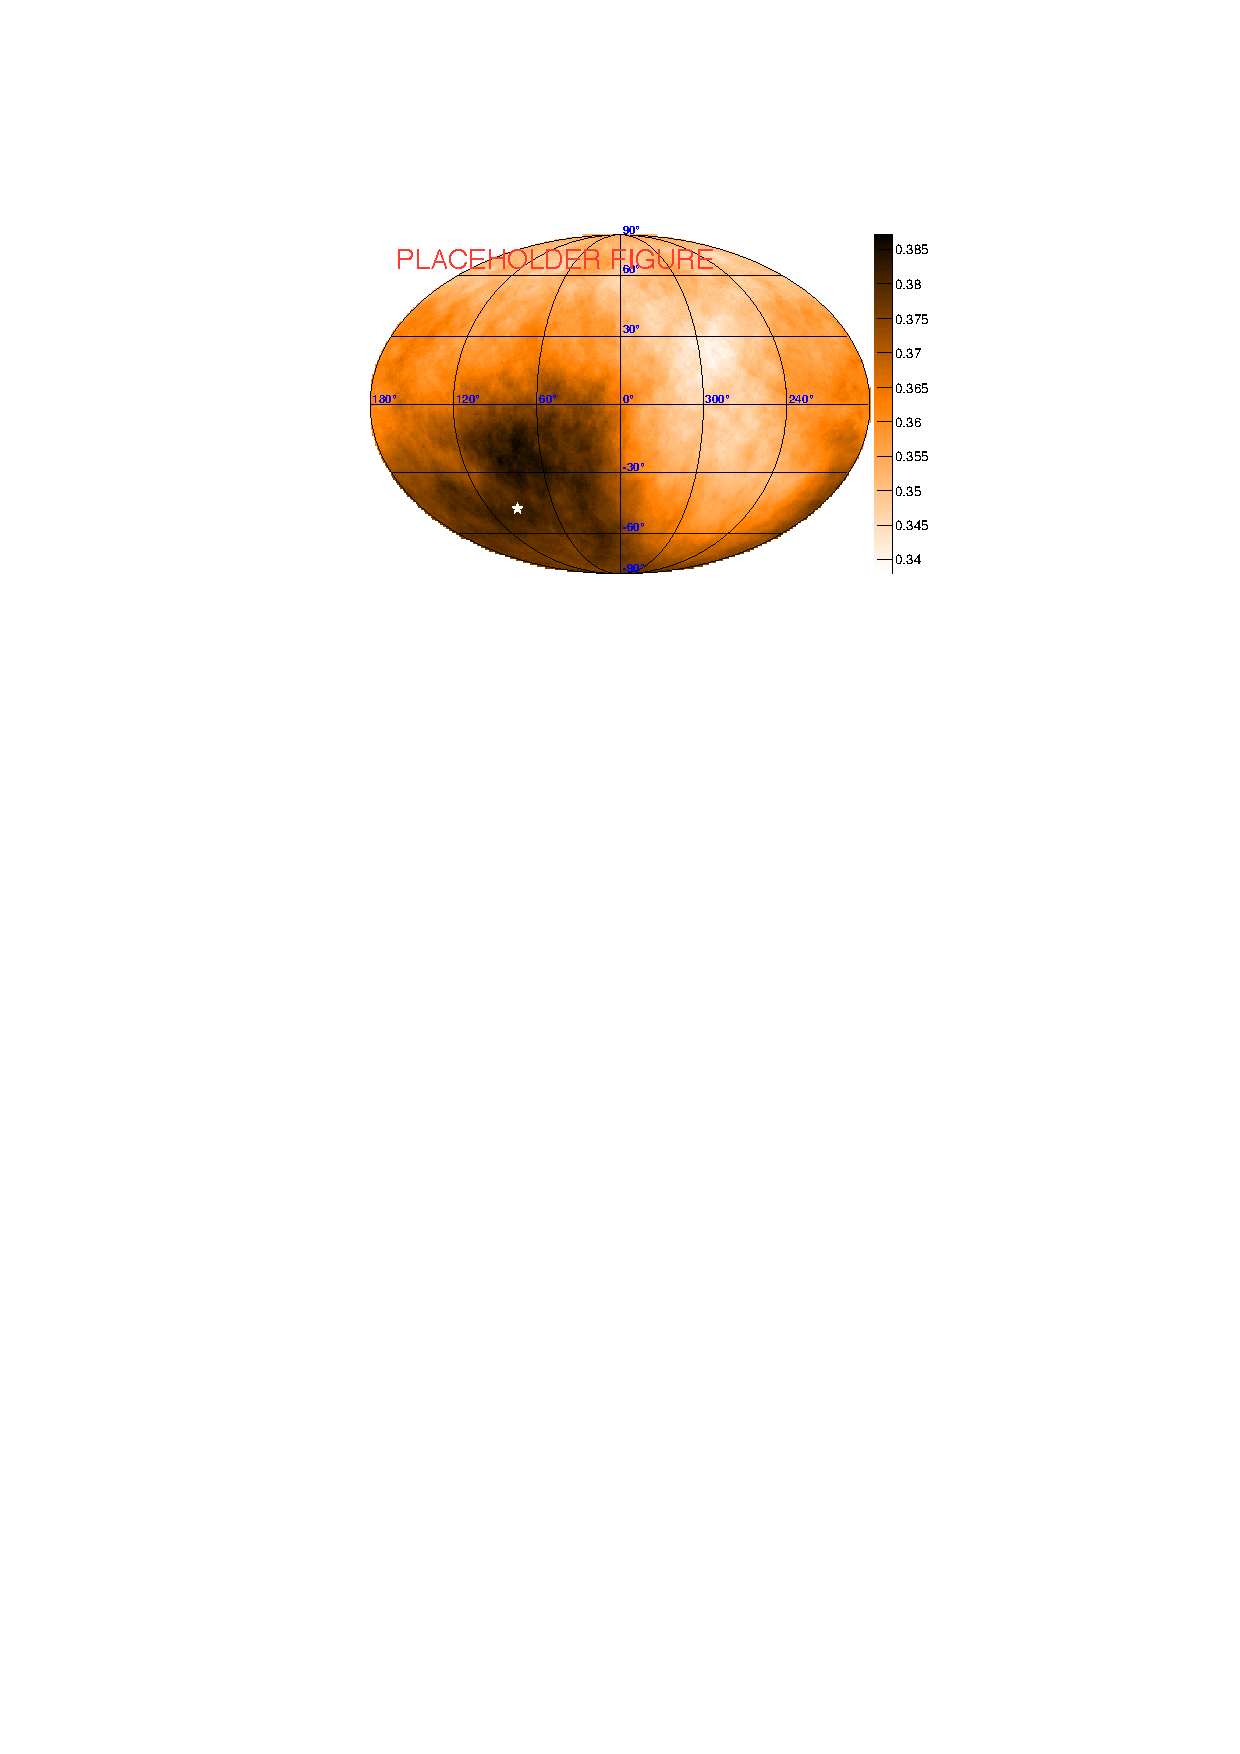
\includegraphics[width=0.6\textwidth]
                    {plots/cosmic-rays/skymap_ta_auger}
    \caption{Anisotropy measurement for cosmic rays of $E > \SI{e19}{\eV}$ by the combined Pierre Auger Observatory and Telescope Array data. The overlapping regions are used to correct for sensitivity differences between the experiments. Only a dipole moment is seen, higher multipoles do not deviate from the expected fluctuations of an isotropic flux at \SI{99}{\percent} confidence level. The color scale units are in \si{\per\kilo\meter\squared\per\year\per\steradian}}
    \label{fig:skymap_ta_auger}
\end{figure}

\begin{figure}
    \centering
    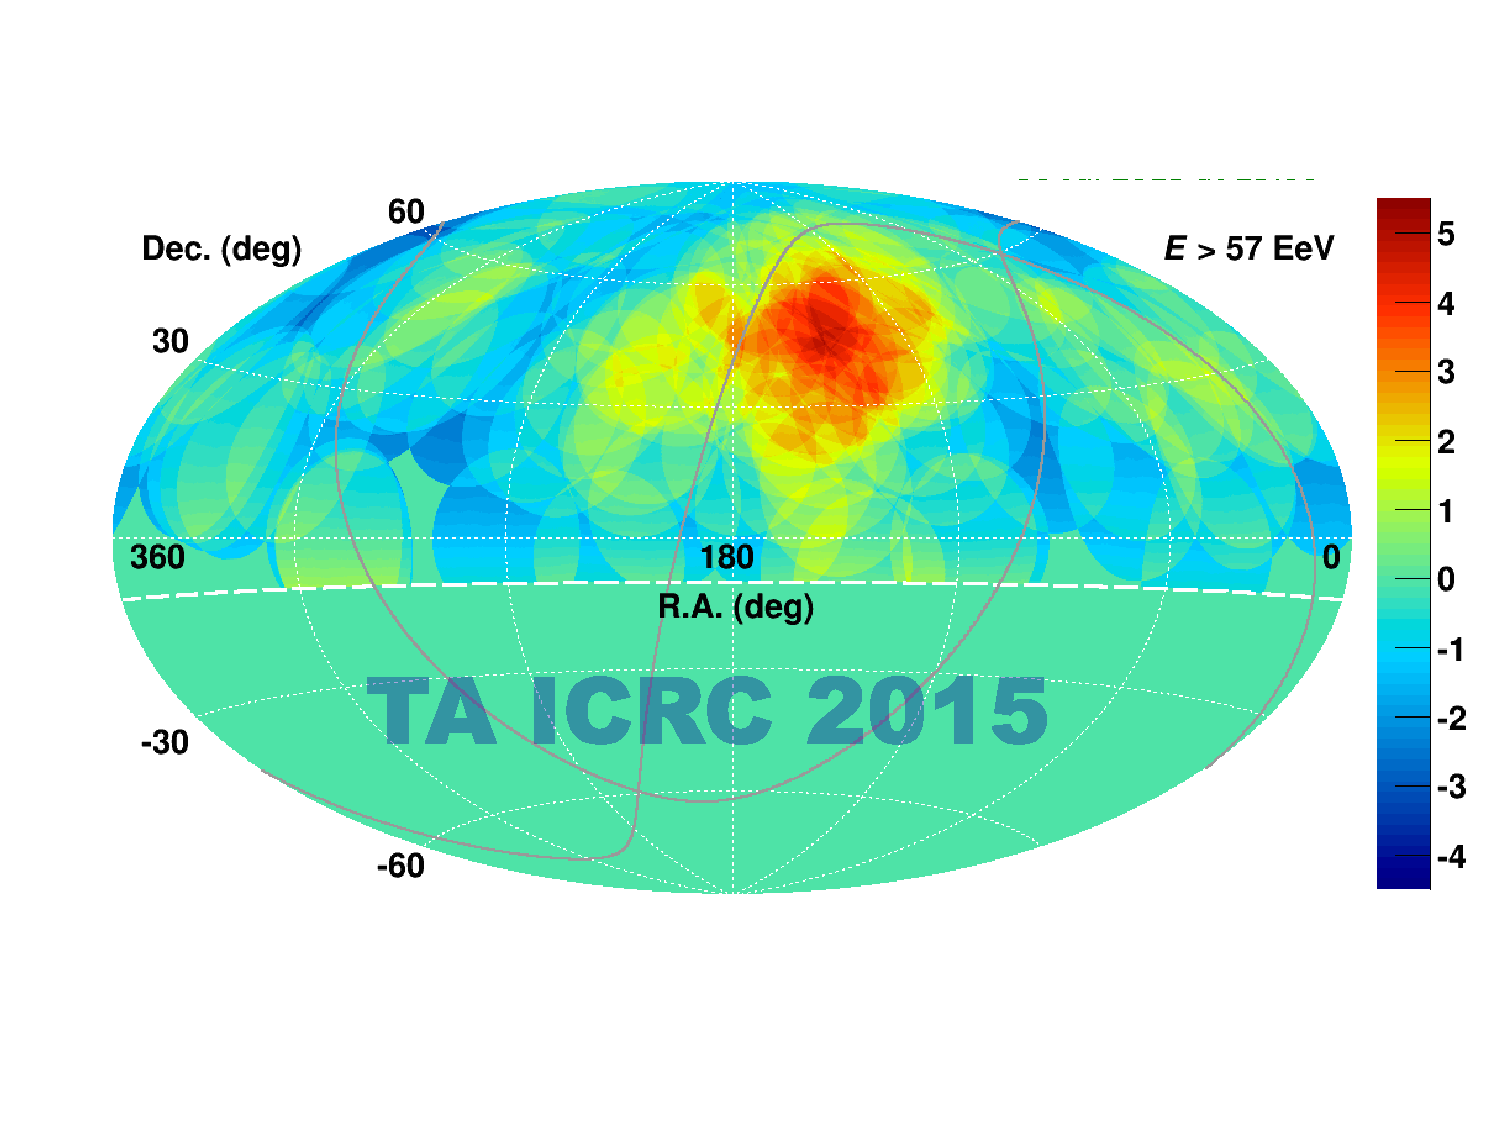
\includegraphics[width=0.6\textwidth]
                    {plots/cosmic-rays/hotspot_ta}
    \caption{Hot spot by TA on mollweide plot, abasi2015]
Anisotropy significance plot for the Telescope Array data for primary cosmic rays of $E > \SI{57e18}{\eV}$. Here a hot spot with a significance of $3.4 \sigma$ is observed. This may indicate a source, but more data is required for a more definite conclusion.}
    \label{fig:hotspot_ta}
\end{figure}

% Highlight some of the features of the high energy spectrum, and that there is some composition information known (light-heavy) but no exact fractions.
In \cref{fig:PDG_28_8_all_particle_spectrum} the height of the spectrum is compressed by scaling the data by $E^{2.6}$. This way certain features are more easily seen. For instance the changes in the steepness of the power law (knees and ancles) are more visible. Composition measurements are less specific for indirect measurements. They do provide an indication for the overall lightness (mostly protons) or heaviness (more biased towards iron) of the composition. It appears that beyond $E = \SI{e18}{\eV}$ the composition becomes heavier \cite{abbasi2015combined}. However, the model predictions upon which these measurements depend are not yet perfect. Improvements to the experiments are planned to increase the exposure and improve the sensitivity to the composition.

\begin{figure}
    \centering
    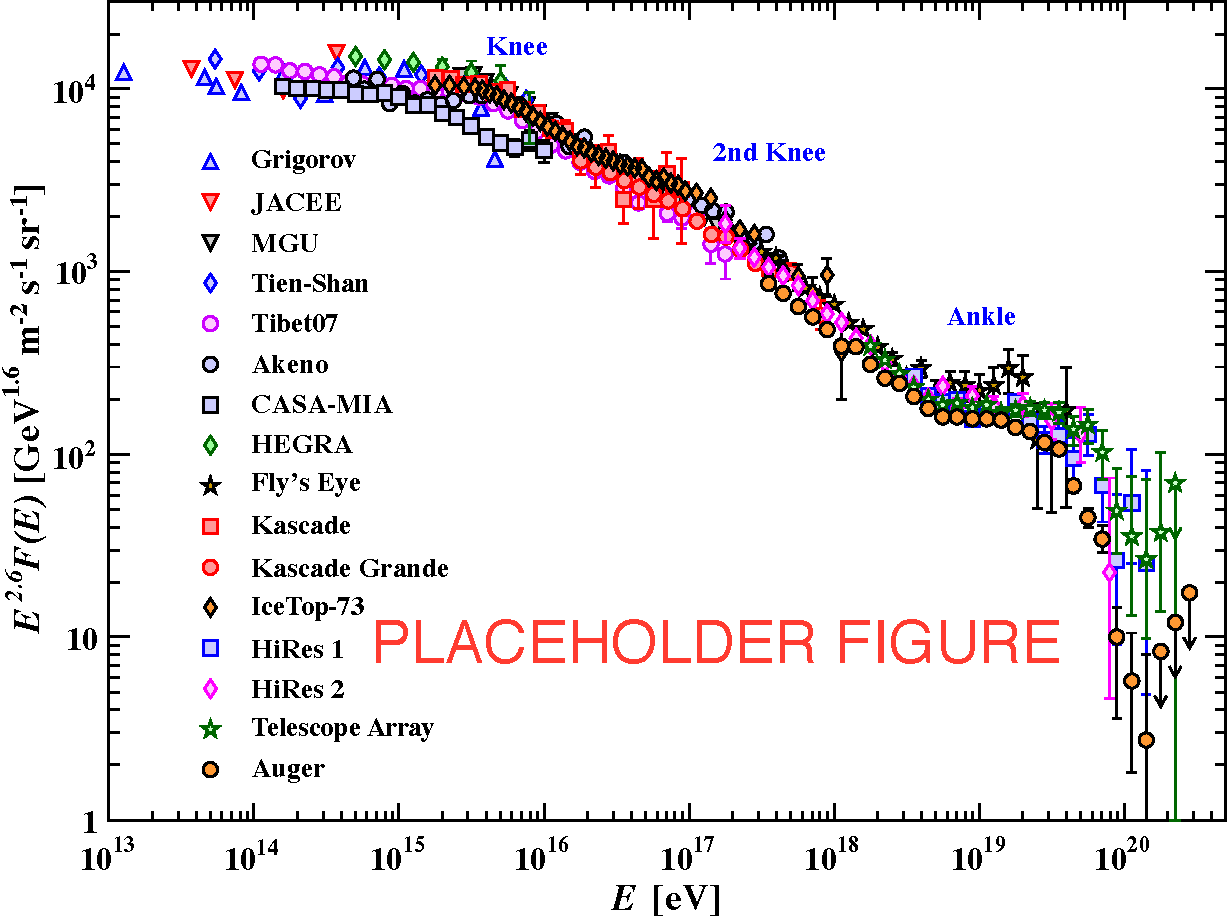
\includegraphics[width=0.6\textwidth]
                    {plots/cosmic-rays/PDG_28_8_all_particle_spectrum}
    \caption{Detailed spectrum at high energies]
The differential flux of cosmic rays multiplied by $E^{2.6}$. This representation of the latest data from cosmic-ray experiments reveals more structure in the spectrum. Little data is available for the highest energy cosmic rays, but limits are set on the maximum rates. The composition of cosmic rays at these energies is not yet known.}
    \label{fig:PDG_28_8_all_particle_spectrum}
\end{figure}


\section{Extensive air showers}
\label{sec:cr:eas}

% Typical hadronic interactions of (hadronic) cosmic rays entering the atmosphere.
% The cross section of such interactions, as known from colliders and cosmic ray experiments.
% Colliders not yet upto highest energies, and different type of interactions.
The first interaction target of incoming cosmic rays are the atoms in the upper atmosphere. The upper atmosphere consists mainly of nitrogen (\SI{78.09}{\percent}), oxygen (\SI{20.95}{\percent}), and argon (\SI{0.93}{\percent}) [fix composition for upper atmosphere, add reference]. Unfortunately collider experiments rarely use these nuclei as collision material. So the exact cross section of interactions between cosmic-rays (anythin between protons a iron) and atomic nitrogen, oxygen, and argon is not known at high energies.

Particle colliders like HERA, RHIC, and SPS [refs, or see figure] have been able to produce collisions center mass energies of several hunderds \si{\GeV}, equivalent to cosmic rays of \SI{e14}{\eV} colliding with a fixed target.

The collider data has been essential for tuning models simulating the interaction in the particle cascades. Using extrapolations models can simulate the expected showers for cosmic-rays of the highest energies. The expected accuracy of the extrapolations becomes less the further they are from the collider data. These colliders provide important data about the hadron production processes in air showers, the cross-sections of the collisions, the multiplicity of secondary high-energy particles and the ratio of neutral to charged particles \cite{pierog2008lhc}.

Fermilab's Tevatron was capable of proton collisions with center of mass energies of \SI{1.8}{\TeV} \cite{abe1994tevatron}, equivalent to collisions of cosmic protons with \SI{2e15}{\eV} against a fixed target. This is approximately the lower energy limit for the KASCADE experiment. However, KASCADE's upper limit was \SI{e17}{\eV}. The LHC is in an interesting energy range; \SI{7}{\TeV} and now upgraded to \SI{14}{\TeV}, equivalent to \SI{2e16}{\eV} and \SI{e17}{\eV} cosmic-ray energies respectively. These are the first time that we have access in colliders to collision energies above the knee in the cosmic-ray spectrum. This also covers the entire energy range of the KASCADE experiment (not KASCADE-Grande). The hadronic interaction models from before the LHC did not properly predict the new LHC data at energies beyond the Tevatron. The EPOS and QGSJETII models have been updated using LHC data from the \SI{7}{\TeV} run. This should provide more accurate results for higher energies. Shower simulations used for this thesis were performed before data from the \SI{14}{\TeV} run had been incorporated into models.

The TOTEM and LHCf experiments at the LHC are placed at the forward regions of the CMS and ATLAS interaction points respectively. These provide the most interessing data for cosmic-ray physics because the interesting products of collisions are those with high pseudorapidity. The LHC runs with p-p collisions most of the time, short periods are run with heavy ions collisions (p-Pb and Pb-Pb). However, for cosmic-ray physics collisions with low-mass ions (oxygen) that are commonly part of the interactions of EAS would be more interesting. Collision data of such interactions would greatly benefit cosmic-ray research.

From p-p collisions the p-Air cross sections can be extrapolated using Glauber theory [reference]. In \cref{fig:pair_crosssection} the proton-Air inelastic collision (i.e. new particles are created) cross section is shown. Measurements by various experiments (points) and predictions by models (lines) are given. At higher energies the models deviate significantly from each other.

\begin{figure}
    \centering
    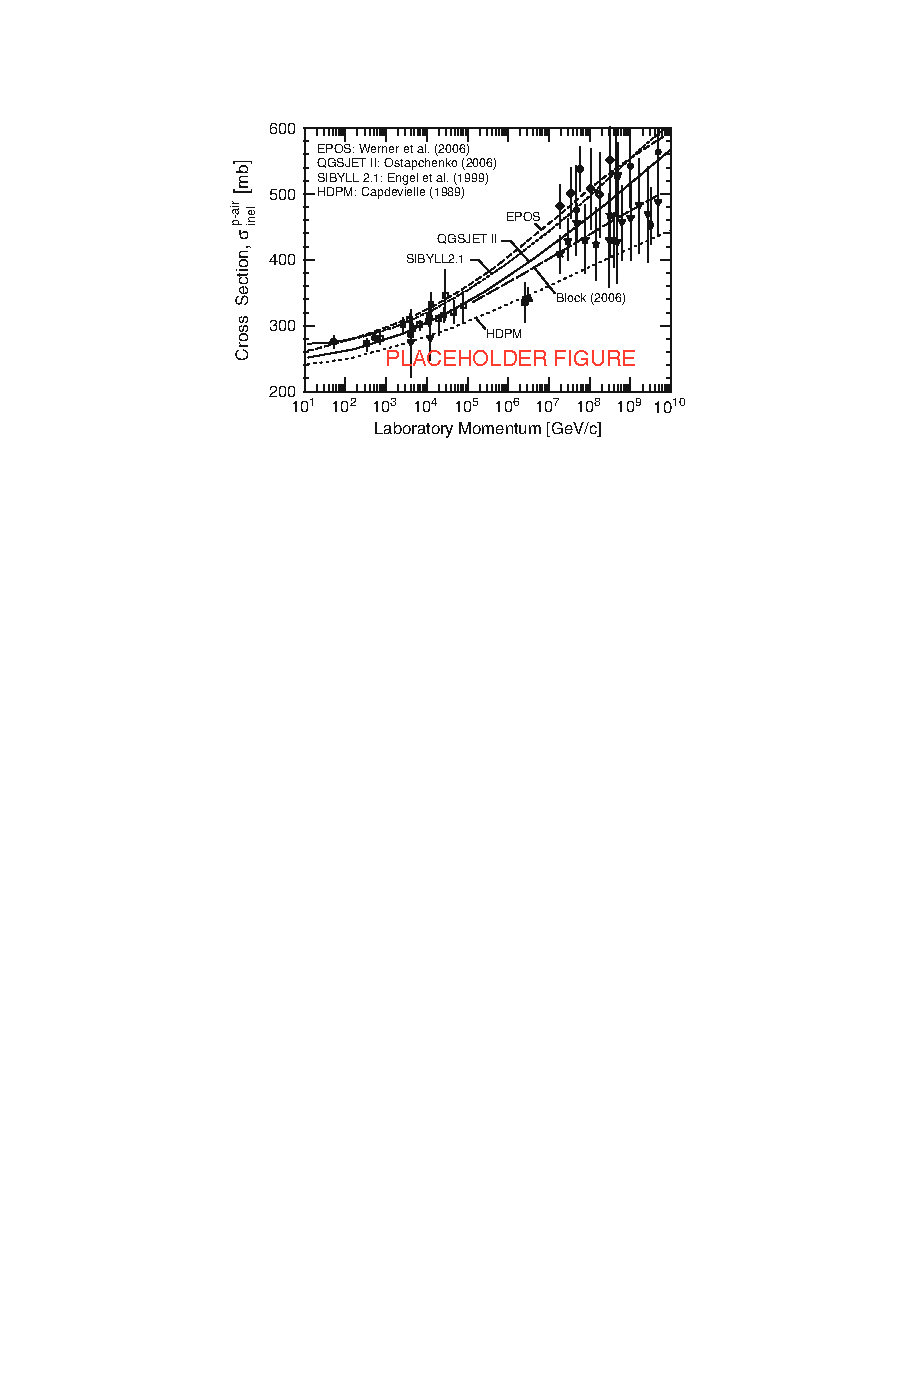
\includegraphics[width=0.6\textwidth]
                    {plots/cosmic-rays/pair_crosssection}
    \caption{Cross section p-Air vs energy, grieder2010]
The measured proton-air cross section determined from cosmic ray measurements of the first interaction altitude. As the energy of the particles increases, so does the cross section. The measurements are within the predicted values from proton-proton cross sections measured in colliders when corrected with Glauber theory.}
    \label{fig:pair_crosssection}
\end{figure}

% Provide the model of the thickness of the atmosphere as a function of the height (as used in CORSIKA).

The density gradient of the atmosphere is the next important factor. The atoms in the atmosphere are the potential targets for the incomming cosmic ray. Earth's atmosphere has been extensively measured and parameterized. As the density increases, so does the probability of a collision. The common way to describe the atmosphere is by giving the column depth, i.e. the amount of material a particle will have passed since it entered Earth's atmosphere. The atmospheric depth is given by

\begin{equation}
    X = \int \rho(h) \diff h
\end{equation}

where $X$ is the atmospheric depth, $\rho$ is the density of the atmosphere as a function of height above ground ($h$). In \cref{fig:atmospheric_depth} the atmospheric depth is shown versus the height above sea level. At sea level the atmospheric depth is approximately \SI{1e3}{\gram\per\meter\squared}. This is the column depth for vertically incoming particles. However, cosmic rays also enter the atmosphere at angles. In this case the path through the atmosphere is longer by approximately $\cos^{-1} \theta$. The resulting column depth is called the slant depth.

\begin{figure}
    \centering
    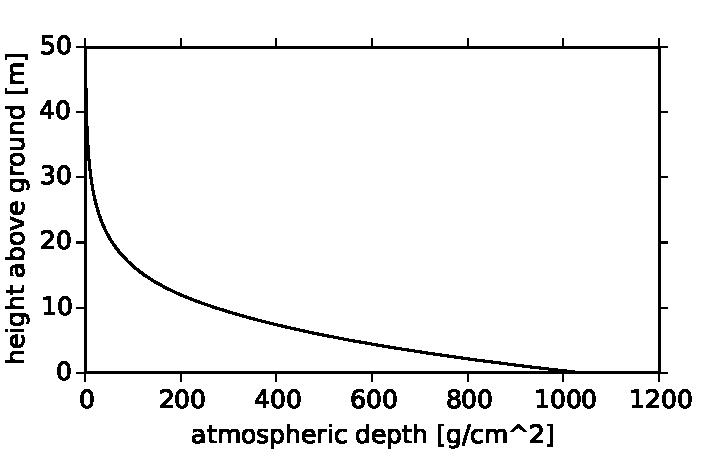
\includegraphics[width=0.6\textwidth]
                    {plots/cosmic-rays/atmospheric_depth}
    \caption{Height vs atmospheric depth, corsika74000]
The atmospheric depth as a function of altitude above ground for typical atmospheric conditions in the Netherlands (CORSIKA model?). The air becomes thinner higher above the ground.}
    \label{fig:atmospheric_depth}
\end{figure}

% The combination of cross section and atmospheric depth gives a distribution for the likely first interaction altitudes.
Monte Carlo simulations using the above described model of the atmosphere and the interaction model QGSJETII-04 give insight in the distribution of the first interaction altitude. In \cref{fig:first_interaction_altitude} the first interaction altitude is shown for vertically incomming proton primaries of $E = \SI{16}{\eV}$. On average the primaries interact interact around \SI{22}{\kilo\meter} above ground where the distribution has a FWHM ~\SI{15}{\kilo\meter}. Cosmic rays of higher energy have a higher mean interaction altitude, since the cross section increases with energy, as shown in \cref{fig:pair_crosssection}.

\begin{figure}
    \centering
    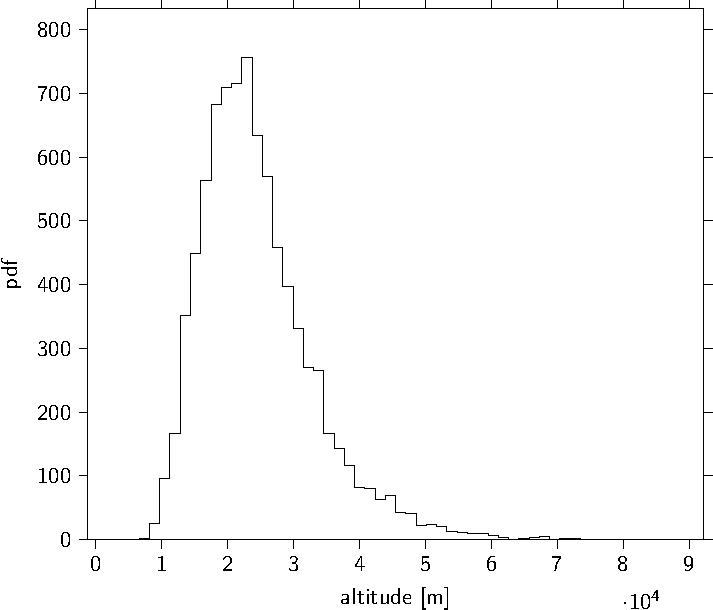
\includegraphics[width=0.6\textwidth]
                    {plots/cosmic-rays/first_interaction_altitude}
    \caption{Distribution of first interaction altitude for showers of certain energy (penetration depth), corsika74000]
Distribution of first interaction altitudes for primary proton cosmic-rays of $E = \SI{16}{\eV}$. From the cross sections a mean free path can be calculated for cosmic rays entering the atmosphere.}
    \label{fig:first_interaction_altitude}
\end{figure}

For inclined cosmic rays higher column depths are reached at higher altitudes, increasing the mean height of the first interaction.

% Explain that these hadronic interactions can produce many secondaries (multiplicty).

The hadronic interaction between the primary hadron and the nuclei produce a number of new particles. The number of generated particles is energy dependend. The mean number of generated charged particles in a proton proton collision is shown in \cref{fig:multiplicity}. These hadronic interactions generate new particles until the energy of the particles falls below the threshold required to produce a pion. They may still undergo interactions at lower energies, but those are of no interest.

\begin{figure}
    \centering
    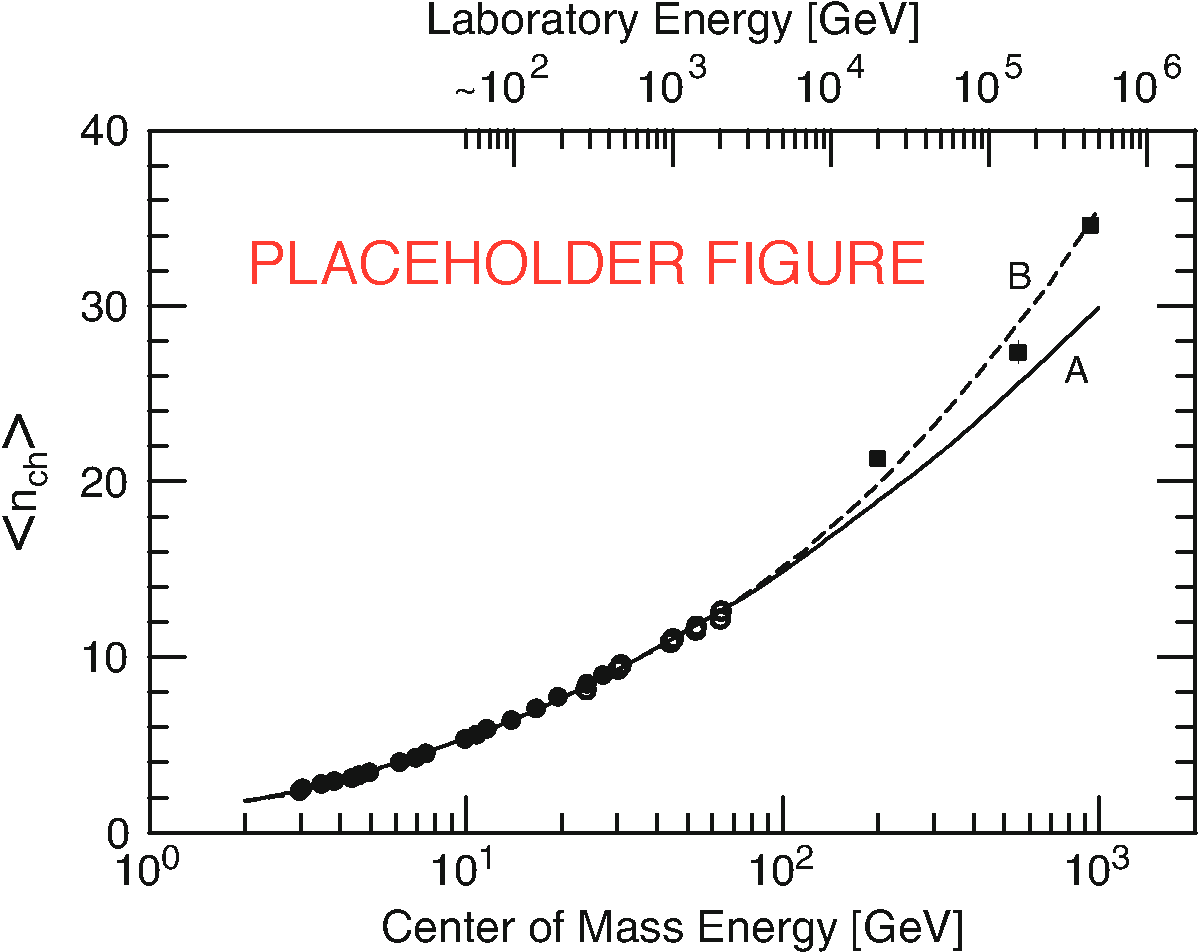
\includegraphics[width=0.6\textwidth]
                    {plots/cosmic-rays/multiplicity}
    \caption{Multiplicity in hard hadron interaction versus energy, grieder2010]
Average secondary particle multiplicty in p-p collisions as a function of the collision energy. The multiplicty increases with the energy of the collision. Results from collider data is shown along with models that try to predict the behavior at higher energies. Predictions vary widely from model to model.}
    \label{fig:multiplicity}
\end{figure}

% Explain what particles are produced and what happens to them.
The most commonly produced particles in these hadronic interactions are light mesons. Neutral and charged pions are most commonly generated. In these hadronic interactions the Baryon number must be conserved. This means that the quark number must remain equal. Each (anti-)quark has a baryon number of $(-)\frac{1}{3}$. Mesons consist of a quark and anti-quark, so have a baryon number of 0. So mesons can 'freely' be added to the output of the interaction. As long as enough energy is available to produce the particles.

\begin{equation}
\HepProcess{\Pproton + \Pproton \to \Pproton + x \Ppiplus + y \Ppiminus + z \Ppizero},
\end{equation}

These reactions are not fully elastic, because new particles are created. However, the incident particle, or parts of it, generally survive and still carry a significant fraction of the energy.

% Explain how energy is transferred into the leptonic part of the shower.
% Particle creation with energy transfer from hadronic to EM
The neutral pions quickly decay (a mean life time of $\tau = \SI{8.4e-8}{\ns}$) via the electromagnetic force into two gamma rays (\SI{98.8}{\percent} of the time).

\begin{equation}
\HepProcess{\Ppizero \to \Pphoton + \Pphoton}.
\end{equation}

Here the baryon number is conserved because leptons, neutrinos, and bosons have a baryon number of 0, equal to that of a meson. The gammas will initiate new electromagnetic cascades. Note that quoted mean lifetimes are for the particle at rest. Given the relativistic nature of the particles in showers, due to the high energies, the mean lifetime are longer in the lab/Earth frame.

The charged pions decay a bit slower ($\tau = \SI{26}{\ns}$) into muons with same charge, and a (anti) muon neutrino.

\begin{equation}
\HepProcess{\Ppiplus \to \APmuon + \Pnum},
\HepProcess{\Ppiminus \to \Pmuon + \APnum}.
\end{equation}

The branching ratio for this process is \SI{99.99}{\percent}, the second most probable decay produces an electron and (anti) electron neutrino.

\begin{equation}
\HepProcess{\Ppiplus \to \APelectron + \Pnue},
\HepProcess{\Ppiminus \to \Pelectron + \APnue}.
\end{equation}

The mean lifetime of the muon is relatively long with $\tau = \SI{2197}{\ns}$. The muons can easily reach ground if they have enough energy because of time dilation and length contraction. Some muons do decay before reaching ground in which case the \Pmuon (\APmuon) produces a electron (positron) and positron neutrino (electron neutrino),

\begin{equation}
\HepProcess{\Pmuon \to \Pelectron + \APnue + \Pnum}, \\
\HepProcess{\APmuon \to \Ppositron + \Pnue + \APnum}.
\end{equation}

In \cref{fig:schematic_shower} a schematic representation of the hadronic interction is seen. After the first interaction many new particles are created. The leading particle (the surviving part of the incident particle) continues towards the ground with a significant part of the energy. It will undergo further interactions, but with lower energy, and thus lower multiplicity.

The dominant interaction for the high energy photons created by neutral pion decay is pair production. The photons must have more energy then the rest mass of the two produced particles, i.e. \SI{1022e6}{\eV} for an electron postitron pair.

\begin{equation}
\HepProcess{\Pgamma \to \Pelectron + \Ppositron}.
\end{equation}

Below this energy Compton scattering and absorption[?] begin to dominate. In Compton scattering the photon recoils of another particle, transfering energy to the other particle.

% Explain Heitler model for EM shower.
Electrons and positrons in the cascade will mainly loose energy via Coulomb bremsstrahlung. In this process the electrons will emit photons when passing close to the nucleus of particles where they are affected by the electric fields of the charges. The mean free path of this process is of the same order as that for the pair production. So on average after each radiation length (mean free path) the photons will undergo pair production while the electrons produce new photons via bremsstrahlung. The number of particles doubles at each stage and the energy is divided over the particles. This simple way of describing the electromagnetic cascade is called the Heitler model.

\begin{figure}
    \centering
    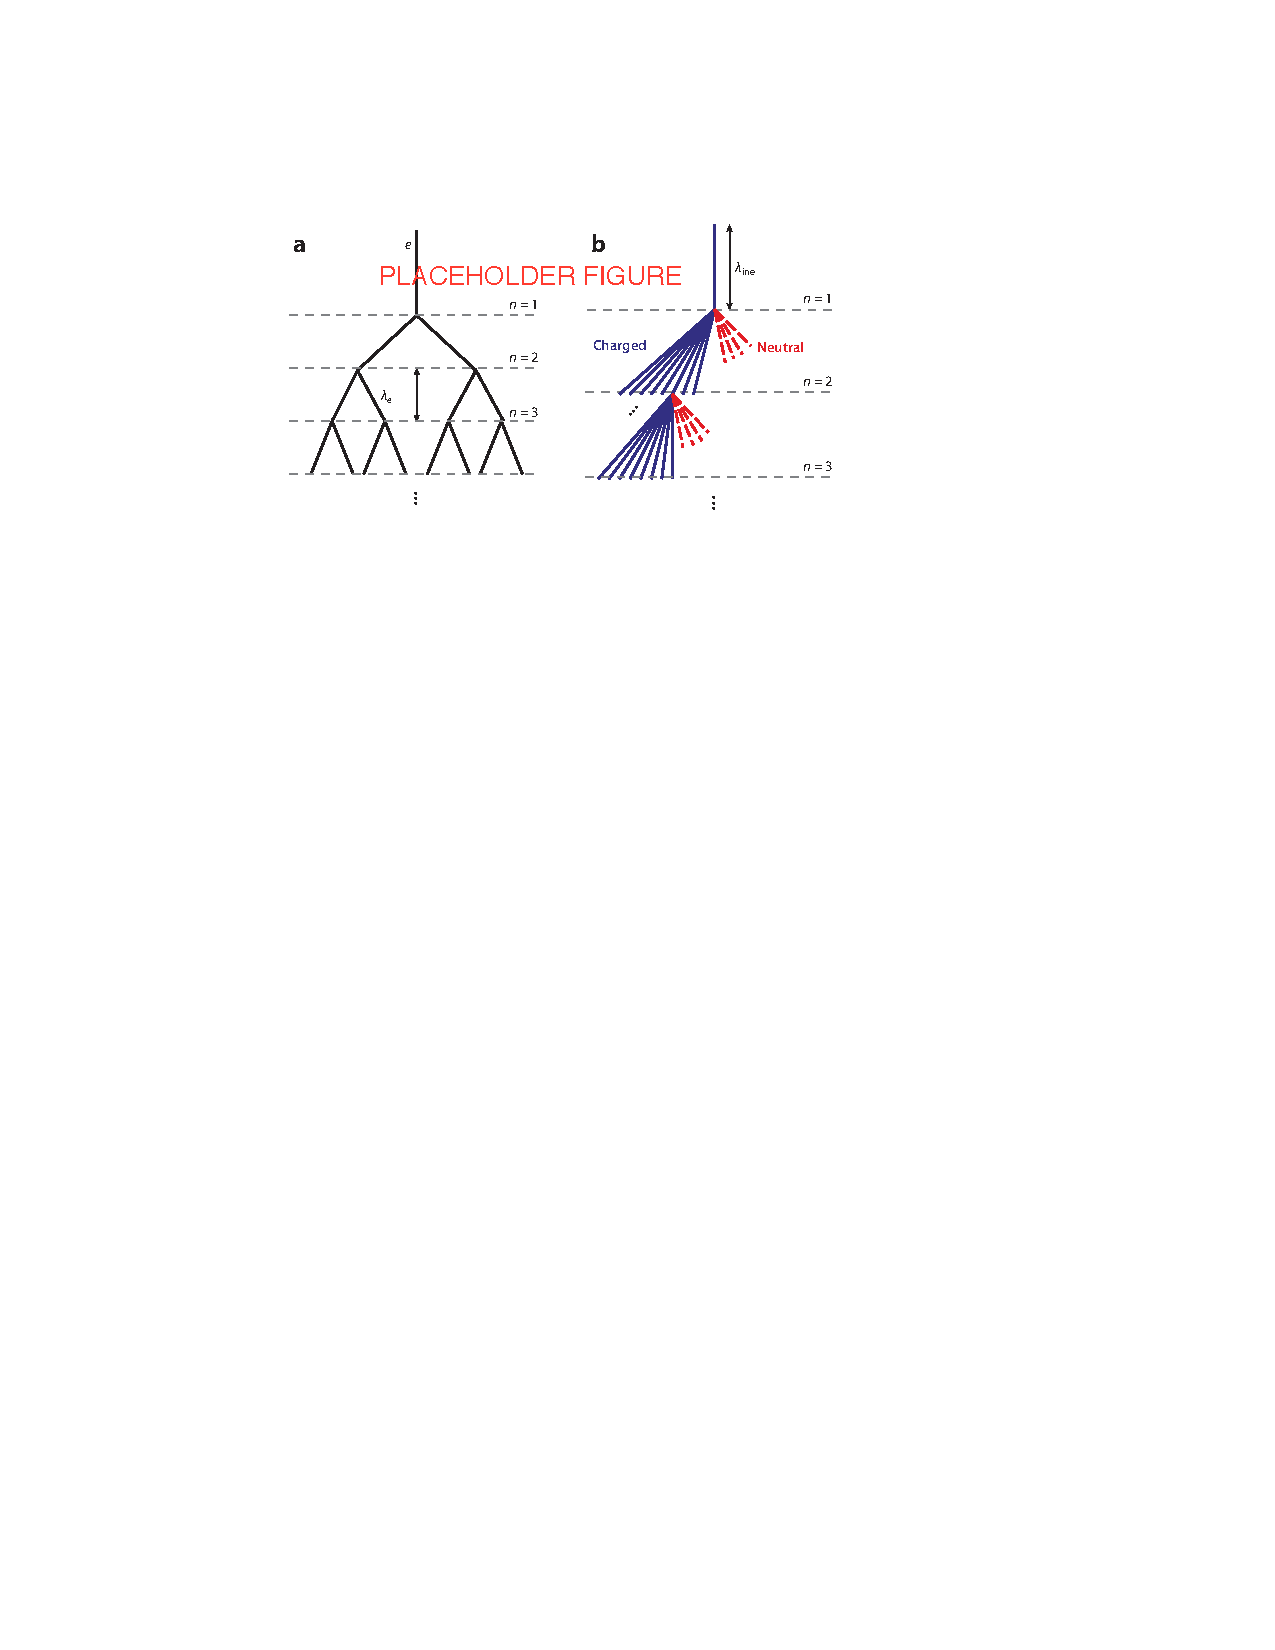
\includegraphics[width=0.6\textwidth]
                    {plots/cosmic-rays/schematic_shower}
    \caption{Schematic shower representation (perhaps separate for hadronic/em), engel2011]
Simple representation of the hadronic and electromagnetic cascades in an air shower. The high multiplicity causes many new charged and neutral particles to be created. The subsequent hadronic interactions are at lower energies and thus, on average, lower multiplicty. After ~6 interaction lengths the shower has reached ground level and most energy will have gone to the electromagnetic shower. For the electromagnetic cascade start when neutral pions or muons decay into gammas or electrons. Gamma's undergo pair creation and electrons (and positrons) emit gammas due to bremsstrahlung. At each radiation length the number of particles doubled, as long as enough energy is available.}
    \label{fig:schematic_shower}
\end{figure}

A full air shower initiated by an incoming hadron will consist of an hadronic component with many electromagnetic subcascades. In the hadronic cascade many pions are produced at different stages. These decay to the muons and gammas. The gammas, and to some extent muons, produce electrons and initiate the electromagnetic cascades.

\subsection{Other observables}

The charged particles reaching ground level are often used to detect the air showers. However, other observables are also created in the shower. The motion of the shower electrons through Earths magnetic field causes them to be slightly deflected, with the positrons being deflected in the opposite direction. In this process radio pulses are created, which can be detected by antennas. Cherenkov radiation is emitted as the fast charged particles move through the atmosphere. The angle of the Cherenkov cone changes with the energy of the shower particles and the height in the atmosphere. Since Cherenkov radiation is emitted along the entire length of the shower information about the development of the shower can be probed. Fluorescence caused by the ionization and excitation of the air causes fluorescence to be emitted along the entire track of the shower. This can also be used to observe the development of the shower from different sides. The fluorescence and Cherenkov radiation is not very bright. Detectors wishing to detect those signals can only operate when there is little background light. That means only at night, no moon, no clouds, no dust in the air, and not to much light polution. These requirements make the duty cycle of these detectors less than \SI{20}{\percent}.


\subsection{Longitudinal}

% This results in a longitudinal profile.
% Particle decay and absorption cause reduction in number of shower particles.
The balance between new particle creation and particle absorption changed as the average energy per particle changes during shower development. When the particles have a enough energy particle production dominates. As energy is spread thin among many particles the absorption will be come more important. Also the decay processed change the balance of hadrons, leptons and gammas. In \cref{fig:longitudinal_profile} the development of the shower as a function of depth is shown. A maximum number of particles in the shower is reached at some point, this is called $X_{max}$. The $X_{max}$ for the different particel types (hadrons, electrons, muons, gammas) are reached at slightly different altitudes.

\begin{figure}
    \centering
    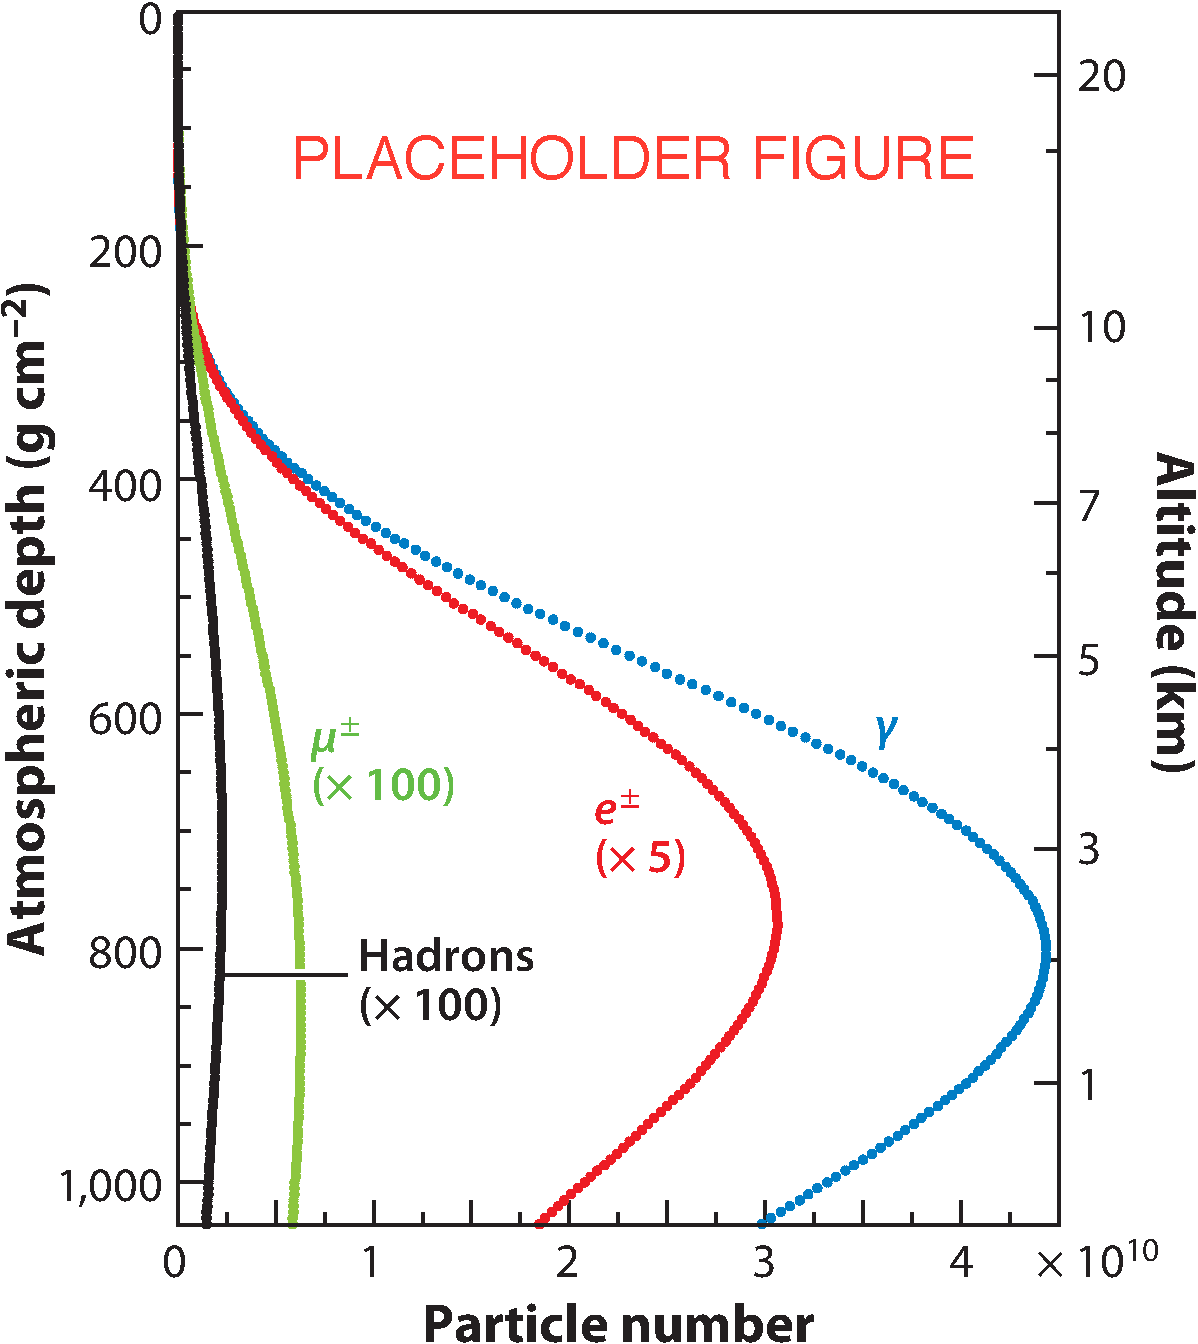
\includegraphics[width=0.6\textwidth]
                    {plots/cosmic-rays/longitudinal_profile}
    \caption{Longitudinal shower profile, with contributions by various particles, engel2011]
The longitudinal shower profile showing the number of particles in the air shower as a function of the atmospheric depth. Different types of particles are shown separately. The depth at which the maximum number of particles exists is called Xmax.}
    \label{fig:longitudinal_profile}
\end{figure}

% The interactions also result in deflections, so the shower expands lateraly.
In the particle interactions and scattering processes the particles emerging from the interaction may have a different direction vector than the incident particle. The transverse momentum of the secondaries mean that the shower extends laterally. Most particles remain close to the shower axis, but low energy ...

% Shower shower profile (CORSIKA).
% Each shower with the same primary energy can develop very differently, chance processes. The size (number of particles) varies for cosmic rays of same energy.

In \cref{fig:shower} all traces of the particles in an air shower are shown. The showers is shown from the side. This is the typical development of a shower. However, the discussed processes are all chance processes. Sometimes the first interaction will be higher, sometimes much later. The multiplicity also differs between collisions of the same energy. The first interactions greatly affect the development of the rest of the shower. In \cref{fig:shower_size_distribution} the total number of leptons reaching ground level (with energy above thresholds) is shown for simulated showers of different energies. All showers are from the zenith. As can be seen the final number of particles varies greatly, spanning about a decade. Showers with a lower point of first interaction will result in larger shower sizes. Note that  here ground level is approximately sea level, at $X = \SI{1080}{\gram\per\centi\meter\square}$, so the shower is diminishing. If the observation level would be around $X_{max}$ the shower sizes would be more consistent.

\begin{figure}
    \centering
    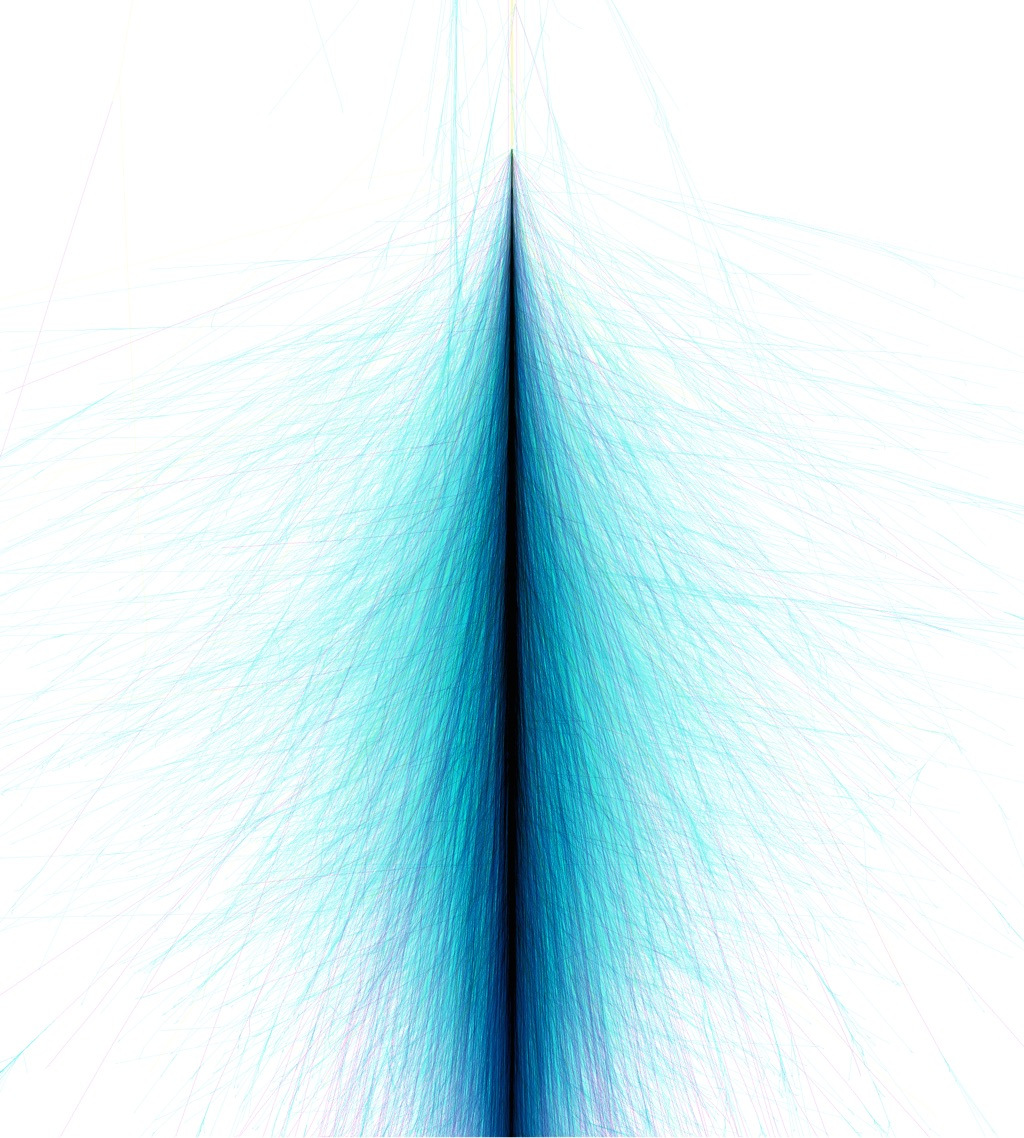
\includegraphics[width=0.6\textwidth]
                    {plots/cosmic-rays/shower.jpg}
    \caption{CORSIKA shower simulation to show spacial development, corsika74000]
Particle tracks of a simulated air shower from a proton with $E = \SI{e16}{\eV}$. The different types of particles are shown with different colors. This shows both the longitudinal and lateral distribution of particles. Motion in the y-direction is ignored.}
    \label{fig:shower}
\end{figure}

\begin{figure}
    \centering
    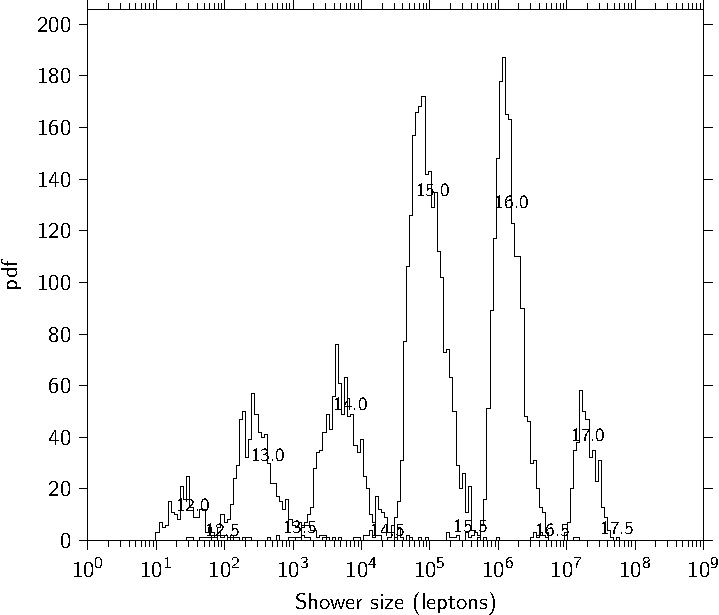
\includegraphics[width=0.6\textwidth]
                    {plots/cosmic-rays/shower_size_distribution}
    \caption{Shower size distributions for showers of various energies, corsika74000]
Number of leptons on ground distributions versus the energy of the primary particle. The variation from shower to shower means that showers will have a different number of particles reaching ground level, eventhough the primary energy was equal. The variations can be as high as a factor 10.}
    \label{fig:shower_size_distribution}
\end{figure}


\section{Shower front}

% What the shower looks like as it reaches ground, how this shape is a result of the various interactions.

Of interest to ground-based experiments is what the observables on the ground are. The focus will be on the leptons and high energy gamma rays which can be efficiently detected. The shower development in the air happens fast, many of the created particles have a lot of energy and move at relativistic speeds. And their direction of motion is approximately equal to the initial incident particle. If a snapshot were made during the development of the shower a 'front' would be seen. The shower front is the shell of particles moving towards ground. The highest density will be at the core of the shower axis, with a lower density towards the edges. The thickness of the shower front will increase at larged core distance because of the different path lengths the particles took to get there will vary more. The front of the shower front is not flat/tangent, at larger core distances the first particles will be delayed relative to the tangent plane of the first particle, again because that particles will have needed to travel a longer distance to get to the sides. Theoretically a causal front exists, a (semi-)sphere with the first interaction at its origin which moves with speed $c$. Since no particle is known to travel faster than light there should be no particle from the shower that reaches ground before the causal front. The expected curvature of the shower front is approximately a sphere. In \cref{fig:schematic_front} these discussed features are shown in a schematic representation of the shower front.

\begin{figure}
    \centering
    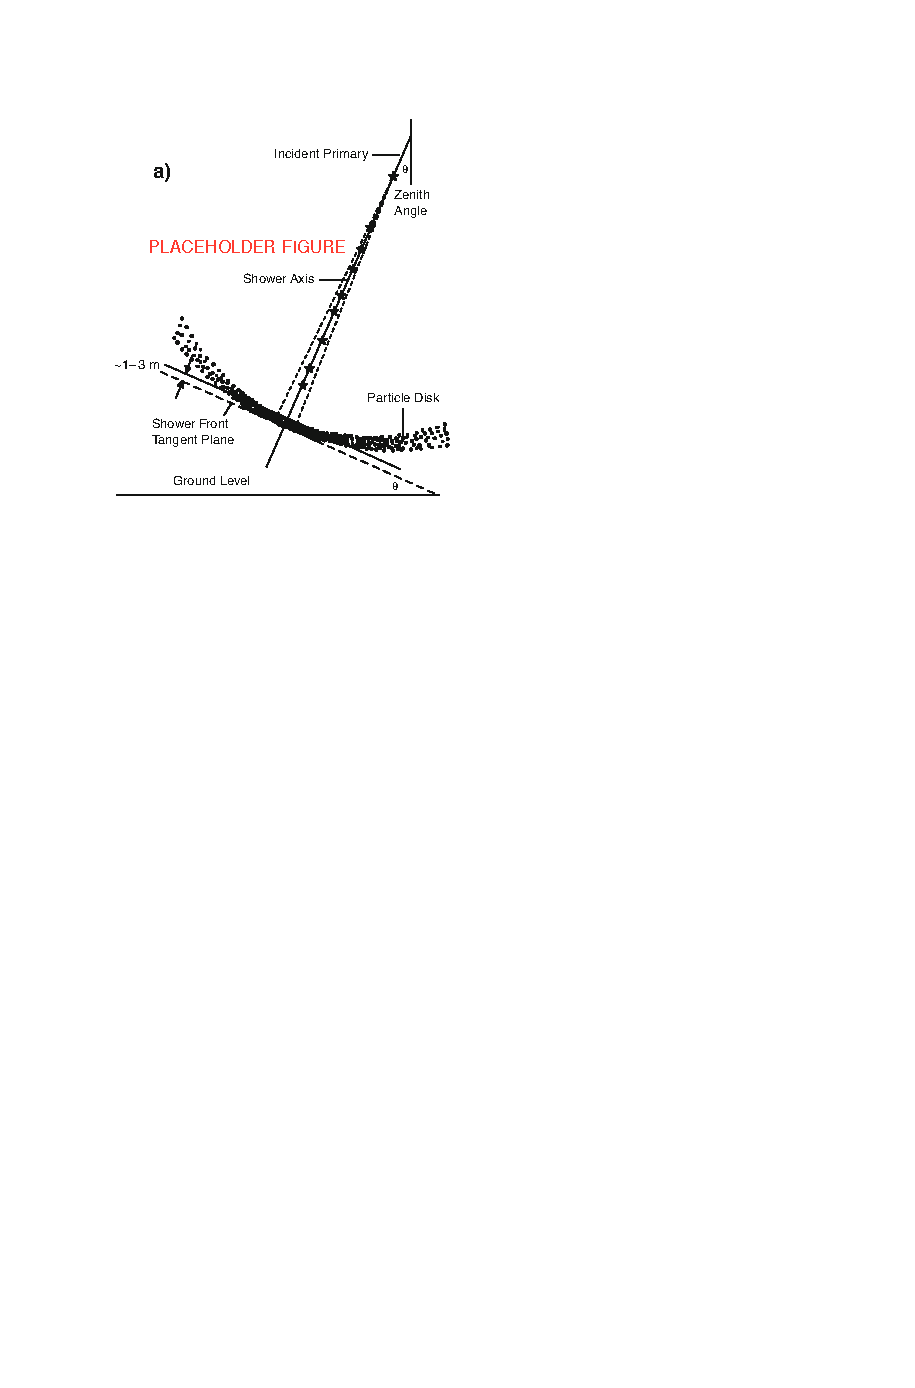
\includegraphics[width=0.6\textwidth]
                    {plots/cosmic-rays/schematic_front}
    \caption{schematic representation of shower front]
A schematic representation of the shower front as it reached ground level. The dots represent shower particles. This is a snapshot in time, so all particles are moving with approximately $c$ to the ground. The particles on the front will reach the ground first followed by those behind. Near the core the density of particles in higher and they are closer to the front. Away from the core the front is curved away from a flat shower front plane. The thickness (rise time) of the front increases with core distance.}
    \label{fig:schematic_front}
\end{figure}

The shower front can be defined in multiple ways, either as a snapshot in time or the front as is passes an observation level. In the first case the $z$ coordinates of particles is relavant, in the second it is replaced by the arrival time $t$. Since particle detectors are fixed at a certain altitude the second definition will be used when refering to the shower front.

% The important distributions related to the shower front.
% LDF for various components, and what influences it.
The particle density at the core of the shower front is highest and then quickly deminishes as the distance increases. In \cref{fig:ldf} the typical particle density as a function of core distance is shown for different particle types. The most common particles are high energy (>\SI{3e9}{\eV}?) gamma rays, followed by electrons, then muons. The density decreases rapidly with increasing distance. The lateral density distribution can be parameterized by a so called lateral distribution function (LDF). Several such parameterizations exist, namely the NKG, KASCADE, AGASA... Some are specifically tuned to experiments, including the atmospheric depth of the experiment, and thus the aproximate shower age [definition?] when showers hit the detectors.

On average the particle density increases with the energy of the primary particle.

- Why this shape

\begin{figure}
    \centering
    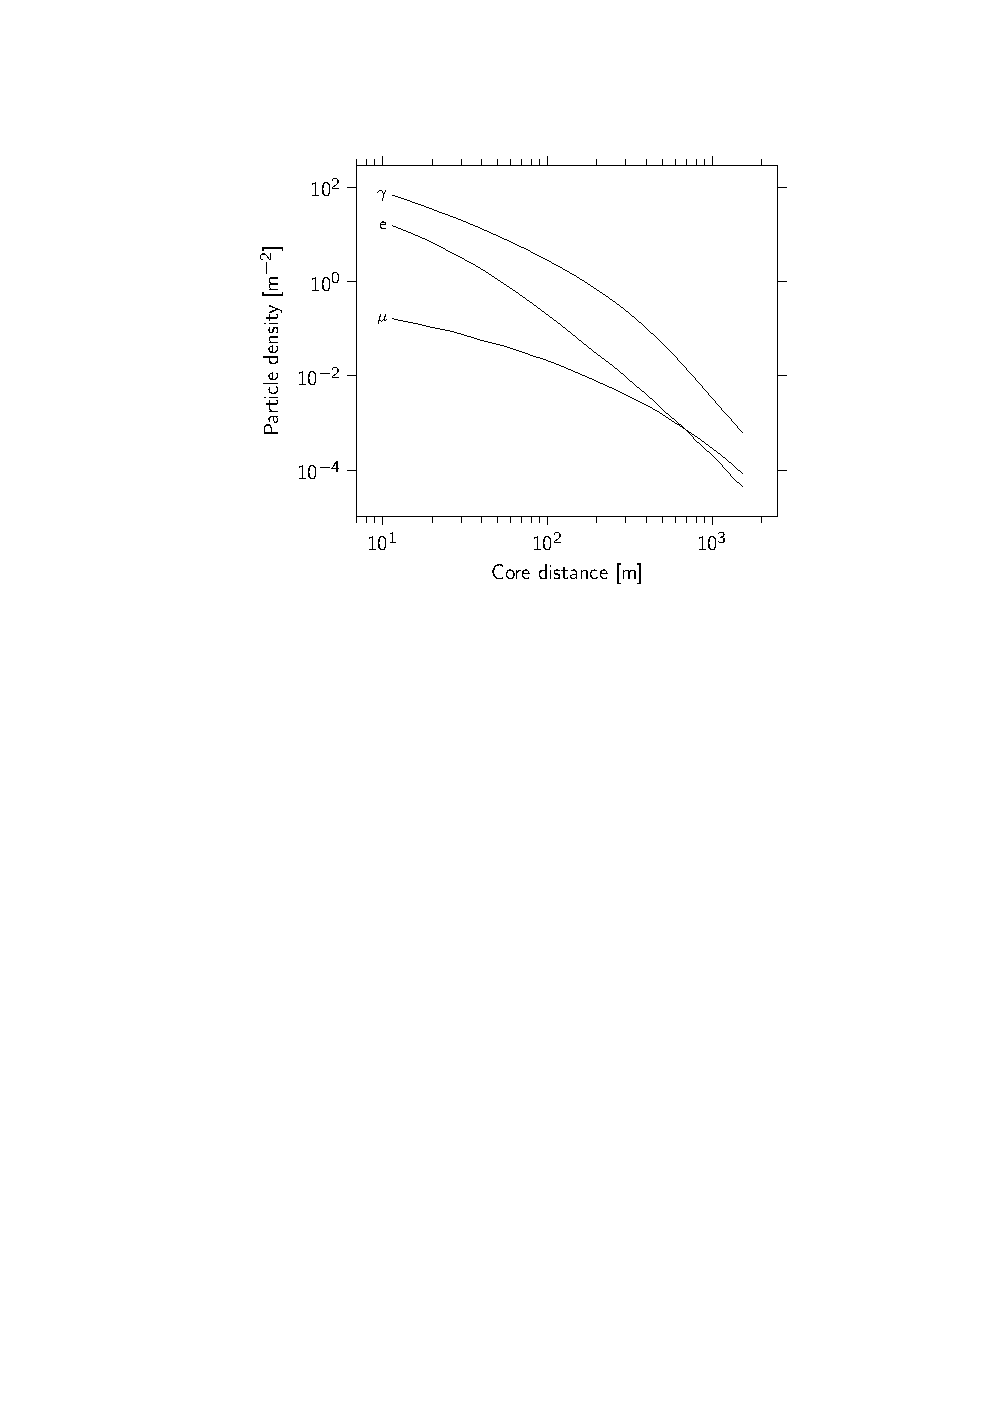
\includegraphics[width=0.6\textwidth]
                    {plots/cosmic-rays/ldf}
    \caption{Lateral density distribution]
The particle density as a function of core distance for a shower of $E = \SI{e16}{\eV}$. The contribution from te different components is shown.}
    \label{fig:ldf}
\end{figure}


\subsection{Temporal shower front}

% At various core distances the temporal profile.
The temporal structure of the shower front can be seen for various core distances in \cref{fig:temporal_profile}. Shortly after the first few particles most of the shower front crosses the obervation level, followed by a long tail of straggling particles. Further from the core the particle density is lower and the spread in arrival times increases.

A hypothetical particle detector would detect many particles if close to the core. The probability is high that one of these particles would be close to the front. At larger distances the density becomes lower, so only a few particles are detected. Moreover, the temporal distribution is much wider so the probability that the particles is further delayed from the front is larger.

\begin{figure}
    \centering
    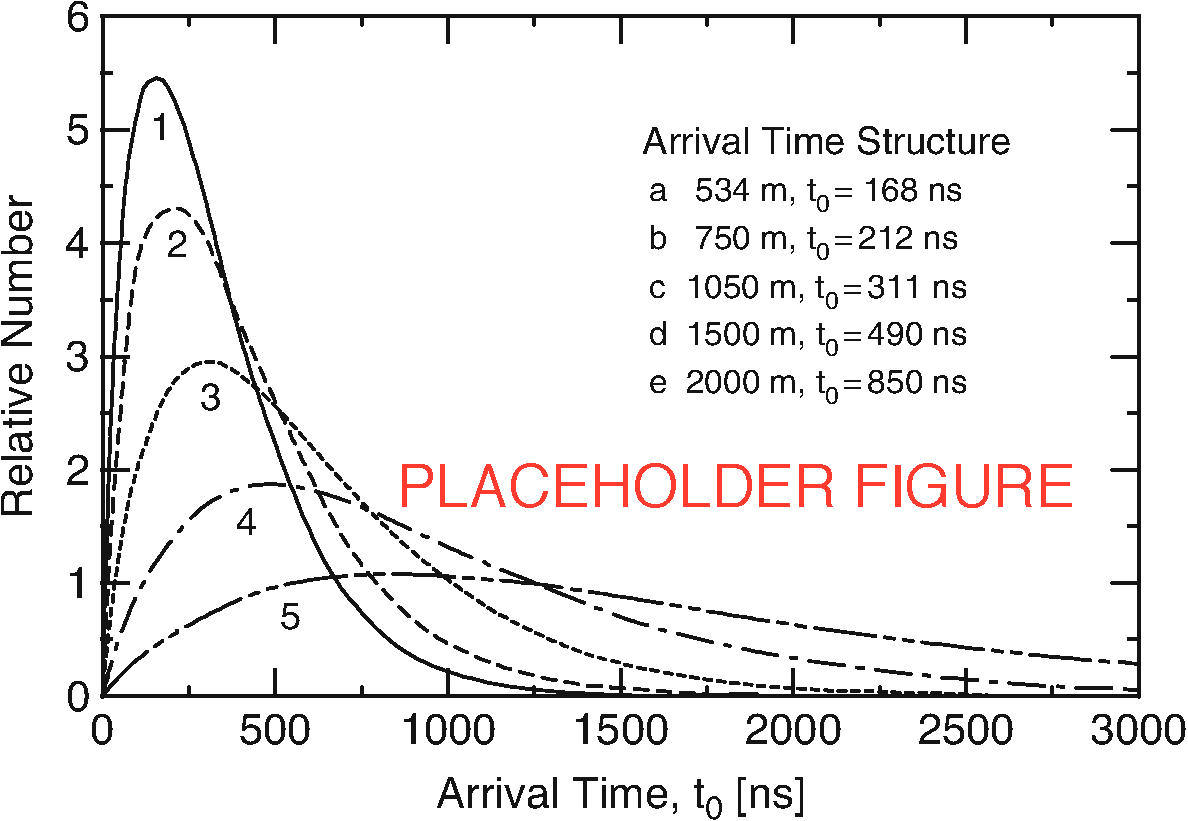
\includegraphics[width=0.6\textwidth]
                    {plots/cosmic-rays/temporal_profile}
    \caption{Temporal structure of shower front, for various core distances]
The temporal structure of the shower front at different core distances for different types of particles. $t = \SI{0}{\ns}$ is the time the first particle reaches ground. Muons arrive first, followed by the gammas and electrons. Each has a long tail of stragglers.}
    \label{fig:temporal_profile}
\end{figure}


- The energy distribution of the particles in the front (see if they are high/low/close to decay).

The energy distributions of the particles on ground... electrons/muons speed...

[Lateral energy distribution, average energy per particle versus core distance]
The (mean particle energy or energy density) as a function of core distance. Close to the code the particles have more energy?

% Explain why muons are earlier than electron/gamma.
% Explain why the front is curved and the thickness of the front varies.
In [add figure temporal per type] the temporal distribution for the various particle types is shown. The muons are typically first, muons are produced in the charged pion decays and then travel uninterrupted to ground. Electrons and gammas on the other hand undergo many interactions before reaching ground. In each of these interactions there is a possibility of gaining transverse momentum (scattering), this means the trace from the particle on the ground back to the initial interaction will be less of a straight line, more jagged. So on average the electrons arrive after the muons. Gammas...


% The relation between the curvature/rise time to other shower properties.


\begin{figure}
    \centering
    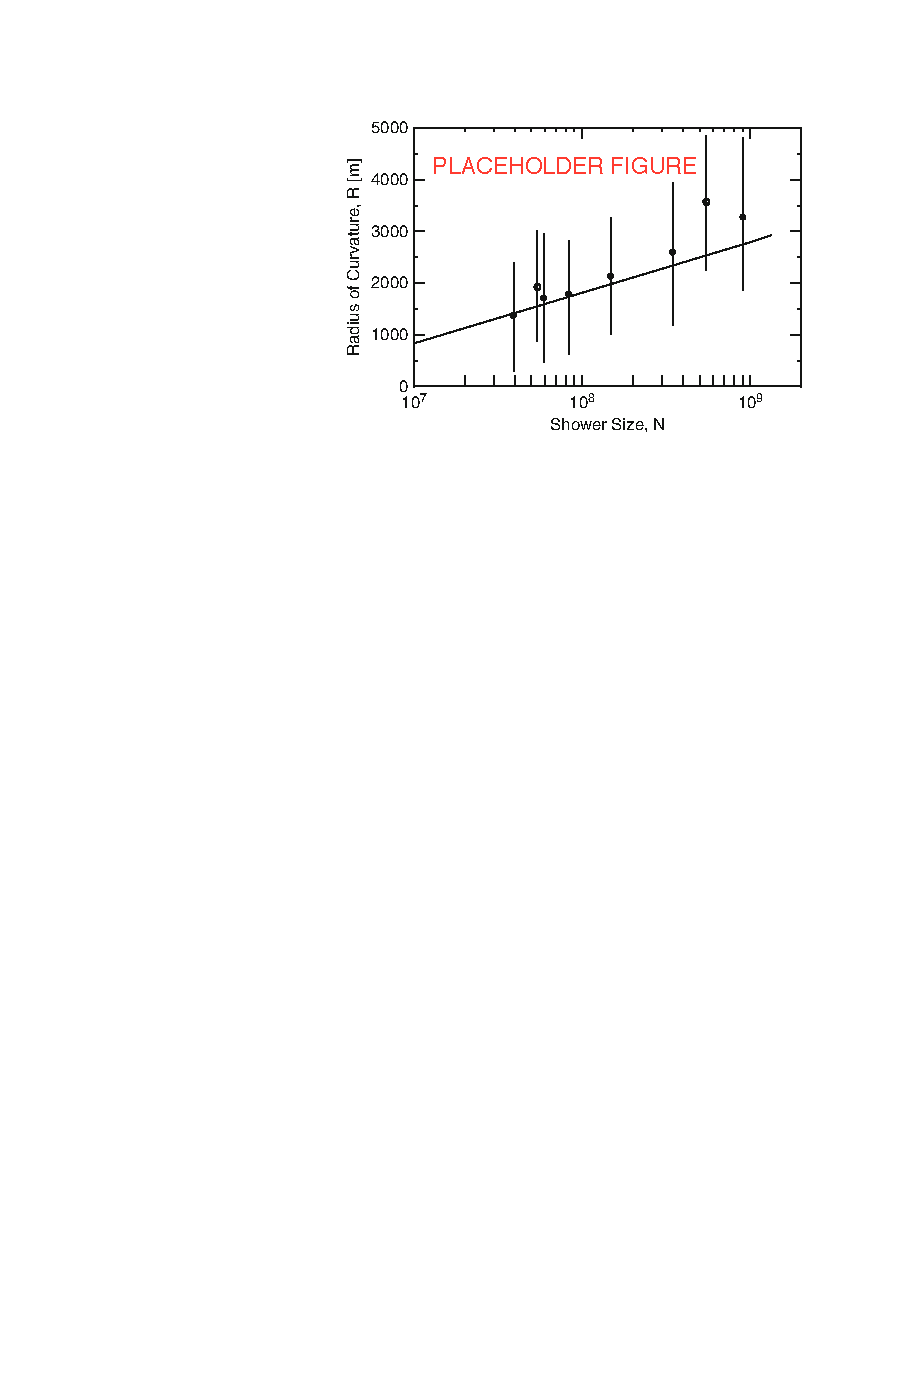
\includegraphics[width=0.6\textwidth]
                    {plots/cosmic-rays/curvature_front}
    \caption{Front curvature as function of size (or interaction altitude)]
The mean shower front curvature as a function of the shower size. The interaction altitude of a shower affects the curvature of its shower front.}
    \label{fig:curvature_front}
\end{figure}

[Front rise time as function of size (or interaction altitude)]
The mean shower front rise time at various core distances as a function of the shower size. The combined rise time for muons and electrons is shown.

